%% --------------------------------------------------------------
%% 
%% Copyright (C) 2001
%% Michael McNeil Forbes
%% mforbes@alum.mit.edu
%% 
%% This file may be distributed and/or modified under the
%% conditions of the LaTeX Project Public License, either version 1.2
%% of this license or (at your option) any later version.
%% The latest version of this license is in
%%    http://www.latex-project.org/lppl.txt
%% and version 1.2 or later is part of all distributions of LaTeX
%% version 1999/12/01 or later.
%% 
%% This program is distributed in the hope that it will be useful,
%% but WITHOUT ANY WARRANTY; without even the implied warranty of
%% MERCHANTABILITY or FITNESS FOR A PARTICULAR PURPOSE.  See the
%% LaTeX Project Public License for more details.
%% 
%% This program consists of the files ubcthesis.dtx, ubcthesis.ins, and
%% the sample figures fig.eps and fig.fig.
%% 
%% This file may be modified and used as a base for your thesis without
%% including the licence agreement as long as the content (i.e. textual
%% body) of the file is completely rewritten. You must, however, change
%% the name of the file.
%% 
%% This file may only be distributed together with a copy of this
%% program. You may, however, distribute this program without generated
%% files such as this one.
%% 

% This Sample thesis requires \LaTeX2e
\NeedsTeXFormat{LaTeX2e}[1995/12/01]
\ProvidesFile{ubcsample.tex}[2012/04/07 v1.70 ^^J
 University of British Columbia Sample Thesis]
% This is the \documentclass[]{} command.  The manditory argument
% specifies the "flavour" of thesis (ubcthesis for UBC).  The
% optional arguments (in []) specify options that affect how the
% thesis is displayed.  Please see the ubcthesis documentation for
% details about the options.
\documentclass[msc,oneside]{ubcthesis}
%
%************************************************
% Optional packages.
%
% The use of these packages is optional, but they provide various
% tools for more flexible formating.  The sample thesis uses these,
% but if you remove the example code, you should be able to exclude
% these packages.  Only standard packages have been described here;
% they should be installed with any complete LaTeX instalation, but
% if not, you can find them at the Comprehensive TeX Archive Network
% (CTAN): http://www.ctan.org/
%

%******** afterpage ***************************
% This package allows you to issue commands at the end of the current
% page.  A good use for this is to use the command
% \afterpage{\clearpage} right after a figure.  This will cause the
% figure to be inserted on the page following the current one (or on
% the current page if it will fit) but will not break the page in the
% middle.
\usepackage{afterpage}

%******** float *********************************
% This package allows you to customize the style of
% "floats"---floating objects such as figures and tables.  In
% addition, it allows you to define additional floating objects which
% may be included in a list similar to that produces by \listoftables
% and \listoffigures.  Common uses include introducing floats for
% programs and other code bits in Compute Science and Chemical Schema.
\usepackage{float}

%******** tocloft *******************************
% This package allows you to customize and define custom lists such
% as a list of programs or Chemical Scheme.  Note: if you use the
% subfigure package, you must specify that you do as an option here.
% The title option uses the default formatting.  We do not use this
% here as the default formatting is acceptable.  Use the float
% package instead unless you need the extra formatting control
% provided by tocloft.
%\usepackage[subfigure, titles]{tocloft}

%******** alltt *********************************
% The alltt package allows you to include files and have them
% formatted in a verbatim fashion.  This is useful for including
% source code from an additional file.
%\usepackage{alltt}

%******** listings ******************************
% The listings package may be used to include chunks of source code
% and has facilities for pretty-printing many languages.
%\usepackage{listings}

%******** longtable *****************************
% The longtable package allows you to define tables that span
% multiple pages.
\usepackage{longtable}

\usepackage{alltt}

%******** graphics and graphicx *****************
% This allows you to include encapsulated postscript files.  If you
% don't have this, comment the \includegraphics[scale=•]{•}graphics{} line following the
% comment "%includegraphics" later in this file.
\usepackage{graphicx}
\usepackage{rotating}

%******** subfigure *****************************
% The subfigure package allows you to include multiple figures and
% captions within a single figure environment.
%\usepackage{subfigure}

%******** here **********************************
% The here package gives you more control over the placement of
% figures and tables.  In particular, you can specify the placement
% "H" which means "Put the figure here" rather than [h] which means
% "I would suggest that you put the figure here if you think it looks
% good."
%\usepackage{here}

%******** pdflscape ********************************
% This allows you to include landscape layout pages by using the
% |landscape| environment.  The use of |pdflscape| is preferred over
% the standard |lscape| package because it automatically rotates the
% page in the pdf file for easier reading.  (Thanks to Joseph Shea
% for pointing this out.)
\usepackage{pdflscape}

%******** natbib ********************************
% This is a very nice package for bibliographies.  It includes options
% for sorting and compressing bibliographic entries.
\usepackage[numbers,sort&compress]{natbib}

%******** psfrag ******************************
% This allows you to replace text in postscript pictures with formated
% latex text.  This allows you to use math in graph labels
% etc. Uncomment the psfrag lines following the "%psfrag" comment
% later in this file if you don't have this package.  The replacements
% will only be visible in the final postscript file: they will be
% listed in the .dvi file but not performed.
\usepackage{psfrag}

\usepackage[T1]{fontenc}

%******** hyperref *****************************
% Please read the manual:
% http://www.tug.org/applications/hyperref/manual.html
%
% This adds hyperlinks to your document: with the right viewers (later
% versions of xdvi, acrobat with pdftex, latex2html etc.) this will
% make your equation, figure, citation references etc. hyperlinks so
% that you can click on them.  Also, your table of contents will be
% able to take you to the appropriate sections.  In the viewers that
% support this, the links often appear with an underscore.  This
% underscore will not appear in printed versions.
%
% Note: if you do not use the hypertex option, then the dvips driver
% may be loaded by default.  This will cause the entries in the list
% of figures and list of tables to be on a single line because dvips
% does not deal with hyperlinks on broken lines properly.
%
% NOTE: HYPERREF is sensitive to the ORDER in which it is LOADED.
% For example, it must be loaded AFTER natbib but BEFORE newly
% defined float environments.  See the README file with the hyperref
% for some help with this.  If you have some very obscure errors, try
% first disabling hyperref.  If that fixes the problem, try various
% orderings.
%
% Note also that there is a bug with versions before 2003/11/30
% v6.74m that cause the float package to not function correctly.
% Please ensure you have a current version of this package.  A
% warning will be issued if you leave the date below but do not have
% a current version installed.
%
% Some notes on options: depending on how you build your files, you
% may need to choose the appropriate option (such as [pdftex]) for the
% backend driver (see the hyperref manual for a complete list).  Also,
% the default here is to make links from the page numbers in the table
% of contents and lists of figures etc.  There are other options:
% excluding the [linktocpage] option will make the entire text a
% hyperref, but for some backends will prevent the text from wrapping
% which can look terrible.  There is a [breaklinks=true] option that
% will be set if the backend supports (dvipdfm for example supports
% it but does not work with psfrag.)
%
% Finally, there are many options for choosing the colours of the
% links.  These will be included by default in future versions but
% you should probably consider changing some now for the electronic
% version of your thesis.
\usepackage[unicode=true,
  linktocpage,
  linkbordercolor={0.5 0.5 1},
  citebordercolor={0.5 1 0.5},
  linkcolor=blue]{hyperref}

% If you would like to compile this sample thesis without the
% hyperref package, then you will need to comment out the previous
% \usepackage command and uncomment the following command which will
% put the URL's in a typewriter font but not link them.
%\newcommand\url[1]{\texttt{#1}}

%******** setspace *******************************
% The setspace package allows you to manually set the spacing of the
% file.  UBC may require 1.5 spacing for microfilming of theses.  In
% this case you may obtain this by including this package and issuing
% one of the following commands:
%\usepackage{setspace}
%\singlespacing
%\onehalfspacing
%\doublespacing

% These commands are optional.  The defaults are shown.  You only
% need to include them if you need a different value
\institution{The University Of British Columbia}

% If you are at the Okanagan campus, then you should specify these
% instead.
%\faculty{The College of Graduate Studies}
%\institutionaddress{Okanagan}
\faculty{The Faculty of Graduate Studies}
\institutionaddress{Vancouver}

% You can issue as many of these as you have...
\previousdegree{B.Sc., The University of British Columbia, 2005}

% You can override the option setting here.
% \degreetitle{Jack of All Trades}

% These commands are required.
\title{TaTAMi}
\subtitle{Taint Tracking for Application Migration}
\author{Lee Alexander Beckman}
\copyrightyear{2012}
\submitdate{\monthname\ \number\year} % The "\ " is required after
                                      % \monthname to prevent the
                                      % command from eating the space.
\program{Computer Science}

% These commands are presently not required for UBC theses as the
% advisor's name and title are not presently required anywhere.
%\advisor{Ariel R.~Zhitnitsky}
%\advisortitle{Professor of Physics}

% One might want to override the format of the section and chapter
% numbers.  This shows you how to do it.  Note that the current
% format is acceptable for submission to the FoGS: If you wish to modify
% these, you should check with the FoGS explicity. prior to making
% the modifications.
\renewcommand\thepart         {\Roman{part}}
\renewcommand\thechapter      {\arabic{chapter}}
\renewcommand\thesection      {\thechapter.\arabic{section}}
\renewcommand\thesubsection   {\thesection.\arabic{subsection}}
\renewcommand\thesubsubsection{\thesubsection.\arabic{subsubsection}}
\renewcommand\theparagraph    {\thesubsubsection.\arabic{paragraph}}
\renewcommand\thesubparagraph {\theparagraph.\arabic{subparagraph}}

\setcounter{tocdepth}{2}
\setcounter{secnumdepth}{2}

% Here is an example of a "Program" environment defined with the
% "float" package.  The list of programs will be stored in the file
% ubcsample.lop and the numbering will start with the chapter
% number.  The style will be "ruled".
\floatstyle{ruled}
\newfloat{Program}{htbp}{lop}[chapter]

% Here is the start of the document.
\begin{document}

%% This starts numbering in Roman numerals as required for the thesis
%% style and is mandatory.
\frontmatter

%%% The order of the following components should be preserved.  The order
%%% listed here is the order currently required by FoGS:        \\
%%% Title (Mandatory)                                           \\
%%% Preface (Manditory if any collaborator contributions)       \\
%%% Abstract (Mandatory)                                        \\
%%% List of Contents, Tables, Figures, etc. (As appropriate)    \\
%%% Acknowledgements (Optional)                                 \\
%%% Dedication (Optional)                                       \\

% NOTES *********************************************
%Notes: whenever I talk about related work, I need to explain why I am different. Someone did this, I'm different this way.
% NOTES *********************************************

\maketitle                      %% Mandatory
\begin{abstract}                %% Mandatory -  maximum 350 words
\paragraph{}
	In this thesis we addressed the question of whether taint tracking could be used to help developers make better application migration decisions. We wanted to determine if detailed dynamic dataflow traces from web applications could support automated analyses, the results of which would help one to better understand applications and guide one in optimizing them.
	
\paragraph{}
	To investigate this problem, we had to build our own taint tracker for Java as none existed which would perform an extensive enough tracing. We then identified a set of useful analyses from a search of the literature and from our own experience with web applications. These analyses were developed to run automatically over taint tracking data, producing output which should be immediately useful to non-expert users.
	
\paragraph{}
	Two real applications were chosen and the analyses applied to them in other to determine two important things. First, that we could write our analyses to automatically identify their targets and produce comprehensible results. Second, that the analysis targets actually existed in real applications.
	
\paragraph{}
	In the end our analyses were mostly successful, in many cases producing clean results which consisely described non-trivial properties of the applications and possible optmizations to them.  By focusing on how data moves through a system, we found a natural fit for understanding its workings. The biggest difficulties manifested as a need for further automation, to take complicated analysis results and simplify them. Even with many challenges, we believe that our techniques are valuable for helping developers, and should be more thoroughly studied.
	
	% Believe in the important of data flow, knowing where each pieces of input goes and where output comes from. This is central.
	
%  Quickly state thesis: taint tracking, previously used primarily in security applications, is useful for discovering various properties of applications which are useful for developers tasks with migrating the application to a new environment or improving it's performance in general. Started with a series of analyses inspired by the literature which we hoped to have success with in taint traces we collected, and also sought to discover unexpected uses for the taint trace data. 
  
%  One thing I need to make clear at some point is that this is not so much about going into great depth on any particular analysis so much as it is about showing that taint tracking supports a wide variety of potentially useful analyses, and these can be done with some success in actual applications. Will want to state here that I tested on two applications, and was able to run successful automated analyses on them with my tools.
  

\end{abstract}

%%\chapter{Preface} % Manditory if any of the conditions are met
%%
%%You must include a preface if any part of your research was partly or
%%wholly published in articles, was part of a collaboration, or required
%%the approval of UBC Research Ethics Boards.
%%
%%The Preface must include the following:
%%
%%\begin{itemize}
%%\item A statement indicating the relative contributions of all
%%  collaborators and co-authors of publications (if any), emphasizing
%%  details of your contribution, and stating the proportion of research
%%  and writing conducted by you.
%%\item A list of any publications arising from work presented in the
%%  dissertation, and the chapter(s) in which the work is located.
%%\item The name of the particular UBC Research Ethics Board, and the
%%  Certificate Number(s) of the Ethics Certificate(s) obtained, if
%%  ethics approval was required for the research.
%%\end{itemize}
%%
%%%%% Sections and subsections etc. in the Preface should in general
%%%%% not be listed in the table of contents, so use the starred form
%%%%% of \section etc.
%%\section*{Examples}
%%Chapter~\ref{cha:apple_ref} is based on work conducted in UBC's Maple
%%Syrup Laboratory by Dr. A.  Apple, Professor B. Boat, and Michael
%%McNeil Forbes. I was responsible for tapping the trees in forests X
%%and Z, conducted and supervised all boiling operations, and performed
%%frequent quality control tests on the product.
%%
%%A version of chapter~\ref{cha:apple_ref} has been
%%published~\cite{Apple:2010}. I conducted all the testing and wrote
%%most of the manuscript. The section on ``Testing Implements'' was
%%originally drafted by Boat, B.  Check the first pages of this
%%chapter to see footnotes with similar information.
%%
%%Note that this preface must come before the table of contents.  Note
%%also that this section ``Examples'' should not be listed in the table
%%of contents, so we have used the starred form: \verb|\section*{Example}|.

\tableofcontents                %% Mandatory
\listoftables                   %% Mandatory if thesis has tables
\listoffigures                  %% Mandatory if thesis has figures
\listof{Program}{List of Programs} %% Optional
%% Any other lists should come here, i.e.
%% Abbreviation schemes, definitions, lists of formulae, list of
%% schemes, glossary, list of symbols etc.

\chapter{Acknowledgements}      %% Optional
Thank Rodger, Eric, and Nima

\chapter{Dedication} %% Optional
Dedicate this thesis to my wife.
%%The dedication is usually quite short, and is a personal rather than
%%an academic recognition.  The \emph{Dedication} does not have to be
%%titled, but it must appear in the table of contents.  If you want to
%%skip the chapter title but still enter it into the Table of Contents,
%%use this command \verb|\chapter[Dedication]{}|.
%%
%%Note that this section is the last of the preliminary pages (with
%%lowercase Roman numeral page numbers).  It must be placed
%%\emph{before} the \verb|\mainmatter| command.  After that, Arabic
%%numbered pages will begin.

% Any other unusual prefactory material should come here before the
% main body.

% Now regular page numbering begins.
\mainmatter

%%%%%%%%%%%%%%%%%%%%%%%%%%%%%%%%%%%%%%%%%%%%%%%%%%%%%%%%%%%%%%%%%%%%%%%%
%	
% A bit too much detail in my writing, can tend to get lost in it.
%
% Upfront have diagram for how my tool operates: phase one, track, phase 2 analysis. Need to remind people of what's going on.
%

%%%%%%%%%%%%%%%%%%%%%%%%%%%%%%%%%%%%%%%%%%%%%%%%%%%%%%%%%%%%%%%%%%%%%%%%


% NOTES *********************************************
%Notes from meeting 20th of August
%-writing is maybe a bit verbose
%-could be a bit clearer. Tighten it up
%-go through paragraphs, find what I can throw away
%-"as such, automated analysis tools have been extremely sought after" -> this is why there has been research in this area.
%
%-took some time to understand what I was telling them.
%-the reader isn't along for the ride, every paragraph has to be about one thing. Each paragraph is about such and such, check. Readers want a kind of A, B, C. 
%
%Try to find what each paragraph is about, and if any sentence disagrees with that, throw it out.
% NOTES *********************************************

\chapter{Introduction} % DIFFICULT

\paragraph{}
Maintaining any sufficiently large application is a difficult task for programmers, especially those who did not write it. In this thesis we focus on web applications, and are concerned with the times in a system's life which require it to change. This is a common event, as has been shown in the history of any popular application which has been around for long enough.

\paragraph{}
The problem is straightforward; a team of developers will implement a system to meet the needs of their users at the current point in time. As we experiment with it later, let us say this system is the RUBiS online auctioning site (think a very simple version of eBay). Eventually, as RUBiS becomes more popular and users want more features (shopping carts, and they're complaining that pages take too long to load), the demand on the application increases. Eventually the original design is insufficient to serve the needs of its users, and some form of migration must happen. New resources are made available for RUBiS to use, such as more servers, but how best to use them? By this time, new developers are on the project, but those who originally designed the system are mostly unavailable to provide support. For these non-experts, making wise decisions about how keep RUBiS up to date is a frustrating and time-consuming process, wrought with many problems:

\begin{itemize}
\item Time is often short
\item Changing application code without being aware of all of its side effects can break it in unexpected ways
\item Real applications are often written poorly, and may not conform to expected patterns
\item The path of data from where it is stored until it gets to users can be long, complex, and very difficult to piece together manually. Knowing these paths are critical to understanding web applications.
\end{itemize}

\paragraph{}
It is here that automation is useful. We want to help these developers by building tools which assist them in understanding their systems more quickly. We even want to automatically make suggestions about how to actually perform optimizations. Tools of this nature have naturally already been researched and developed, and ours represents further exploration into this area. The model of such systems is as follows:

\begin{itemize}
\item Automatically collect data about how applications works. This can be done statically, looking at the code, or dynamically, monitoring the runtime operation of the program.
\item Use this data to build a representation of the application that can be analyzed. This is often a graph model where the application is thought of in terms of components (nodes) which are connected if the data shows a meaningful interaction between them (one component calls another, they exchange data, etc).
\item Run algorithms over the representation (rather than the application itself), to discover properties of it or find ways to optimize it.
\item Map these properties and optimizations back to the original applications, helping developers to better understand and improve them.
\end{itemize}

%- problem statement is going to introduce the problem of migrating an existing application, understanding it, having developers work with it.
%- we believe that taint tracking / dynamic information flow tracking / dataflow tomography can be used to support this process. The interesting thing is that we believe it can support a variety of analyses
%
%
%DISTILLED OUTLINE:
	
% NOTES *********************************************
%Notes: should just say the problem outride. Want to focus more on my particular thread of research. Too much in the larger story, risk losing reader in first few sentences. Really want to start off in a focused manner. It's not a story, should get to the point quicker.
%
%Notes: Really just need to refine this bulk of text.
% NOTES *********************************************

	
\section{Origins of Research}
	
\paragraph{}	
The TaTAMi project is a system which uses dynamic information flow tracking (DIFT) support a variety of analyses for Java web applications.  DIFT is a technique where data is tainted (or tagged) so that its progress can be tracked throughout a system, allowing one to see what parts of the system certain data interacts with and how new data is derived from existing data. The method has been used almost exclusively in the security domain. By tagging untrusted data such as user input, DIFT systems can raise alerts if that data ever propagates to a location it should not, like a config file. We realized that for many of the analyses that we wanted to perform, knowledge of the flow of an application's data throughout its components was key. We anticipated that a heavy-weight variant of taint tracking, dataflow tomography, could extract data which would support many analysis cases.

\paragraph{}
The analyses in question were inspired by works focusing on various forms of dataflow optimization. These include application partitioning, which seeks to split programs into functional pieces and optimally distribute them, and works such as the Fluxo system \cite{Kiciman2010}. Fluxo provided a series of automatic analyses which could be performed over dataflow graph representations of programs, including discovering caches, finding opportunities to delay computation to lower latency, and differentiating between stateful and stateless components. Many of the analyses developed for TaTAMi were derived from those presented in the Fluxo paper, though TaTAMi operates under considerably fewer constraints, as will be discussed later.	
	
\section{Motivating Example}

\begin{figure}[ht]
  \begin{center}
    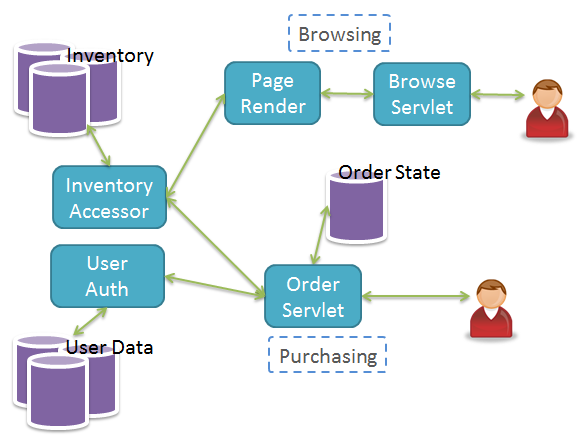
\includegraphics[width=0.6\textwidth]{figs/cap1.eps}
    \caption[Example web store architecture.]{\label{fig:cap1} Example web store architecture.}
  \end{center}
\end{figure}

\begin{figure}[ht]
  \begin{center}
    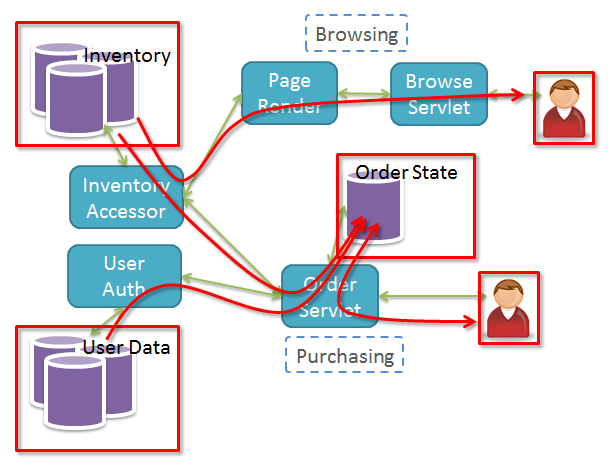
\includegraphics[width=0.6\textwidth]{figs/cap2.eps}
    \caption[Sample dataflow for web store.]{\label{fig:cap2} Sample dataflow for web store.}
  \end{center}
\end{figure}

\begin{figure}[ht]
  \begin{center}
    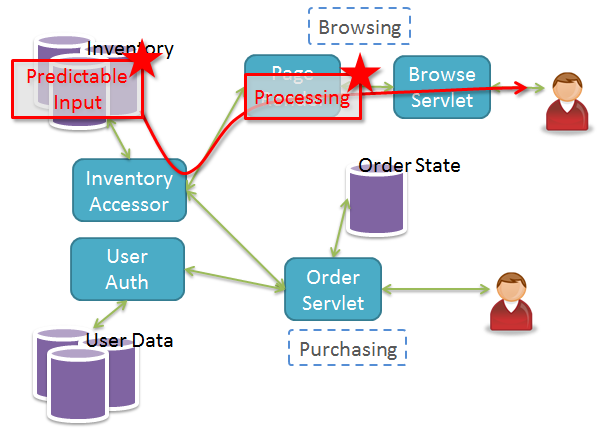
\includegraphics[width=0.6\textwidth]{figs/cap3.eps}
    \caption[Dataflow indicative of possible caching opportunity.]{\label{fig:cap3} Dataflow indicative of possible caching opportunity.}
  \end{center}
\end{figure}

\begin{figure}[ht]
  \begin{center}
    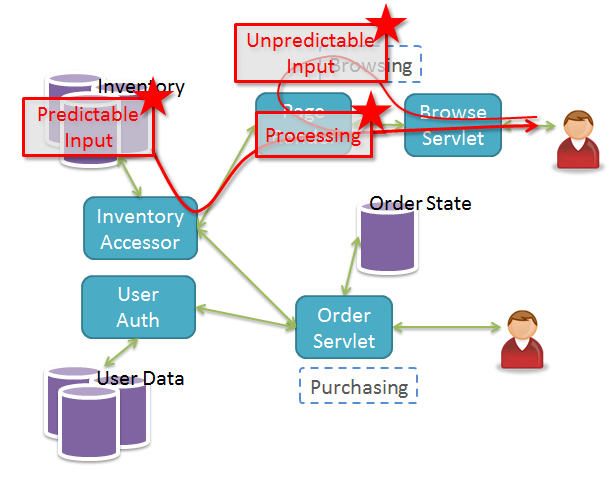
\includegraphics[width=0.6\textwidth]{figs/cap4.eps}
    \caption[Dataflow indicative of sources to be careful of when implementing a cache.]{\label{fig:cap4} Dataflow indicative of sources to be careful of when implementing a cache.}
  \end{center}
\end{figure}

\begin{figure}[ht]
  \begin{center}
    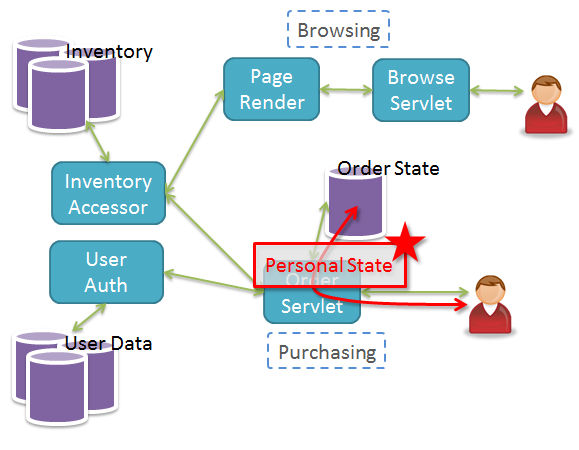
\includegraphics[width=0.6\textwidth]{figs/cap5.eps}
    \caption[Simple dataflow indicating peristent state which is shared with only one user.]{\label{fig:cap5} Simple dataflow indicating peristent state which is shared with only one user.}
  \end{center}
\end{figure}	

\begin{figure}[ht]
  \begin{center}
    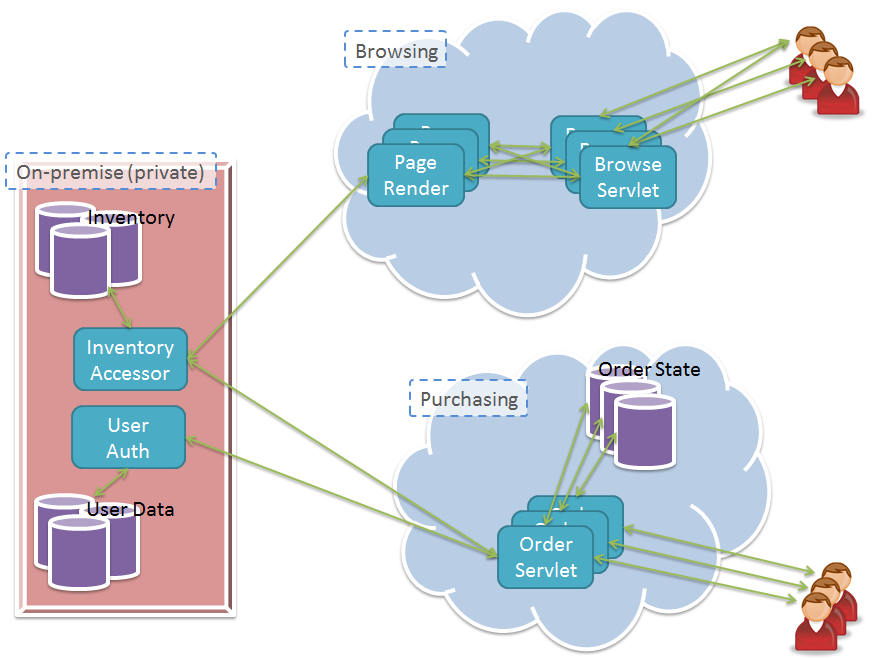
\includegraphics[width=0.6\textwidth]{figs/cap7.eps}
    \caption[Example partitioning of application.]{\label{fig:cap7} Example partitioning of application.}
  \end{center}
\end{figure}
	
To motivate the TaTAMi system and illustrate the natural fit of dataflow tracking to the problem at hand, consider the following:

\subsection{The System}

Presented is a simple online shopping site, the basic architecture of which is given in Figure~\ref{fig:cap1}. The system has back-end data stores for shop inventory and user account info and the logic to access them. For interacting with the site, there are two front-end components: the browsing component which accepts requests from the user to fetch shop items for display, formatted by the page render component; and the Purchasing component, which allows users to maintain a 'shopping cart' list of items they wish to buy and ultimately bill an order to their account. 

\subsection{The Problems}

Problem scenarios are as follows:

\begin{itemize}
\item More users begin using the site. The servers where the Browsing component resides are not fast enough and computations to render pages begin to get backed up.
\item The development team has been asked to move the Purchasing component into the cloud, but the environment there only allows for stateless programs.
\item The network link between the back and front-end components is carrying large amounts of data, and its maximum capacity may soon be reached.
\end{itemize}

\paragraph{}
To start, developers should have an overall picture of how the system works, or at least the part of it they are working on. As stated, we believe that capturing the dataflow of this system will naturally support developers in this effort. Figure~\ref{fig:cap2} presents a possible dataflow graph for the system that our tool would obtain. This is very high level, the arrows indicating that data is communicated from component to component along them. The points to note here are the flow of shop item data from the Inventory database through the Browsing system to the user, and the flow of data from the back-end stores and user input into the 'Order State' shopping cart data. This view focuses immediately on how the application ferries and transforms data throughout its components, the key function of most web applications. It allows a developer to quickly answer the important question: "where did this output come from?"

\paragraph{}
The first optimization to consider, given that the Browsing component is backed up with excessive computation, is precomputation and caching. Consider Figure~\ref{fig:cap3} and Figure~\ref{fig:cap4}, which outline two possible dataflow cases. The first shows how the dataflow could indicate that the data used to generate responses to user browse requests are entirely from predictable sources. Say that browsing involves simply displaying all of the item names, and the set of available items rarely changes, then the output browsing page would remain the same for long periods. The application could potentially be optimized by pregenerating the browsing page and serving it directly to the user, rather than going to the database and running the rendering code. 

\paragraph{}
Figure~\ref{fig:cap4} shows an alternate dataflow where taint tracking indicates that user input flows into the computation for the browsing page. Such could arise, say, if the user supplies some filters to search for items. The input may be very unpredictable, such as for a free text search, and thus the output browsing page may be unpredictable and a poor candidate for any kind of precomputation. On the other hand, if the user input occurs over some reasonably predictable range, such as if the items were being filtered over a set range of categories, the various output browsing pages may be good candidates for caching. An automated analysis could point this out, and a developer is aided in applying this performance improving optimization, knowing which data sources to use for cache keys (user input parameters) and which to check for cache invalidation (the Inventory database).

\paragraph{}
The next concern is moving the Purchasing component into the cloud, to make use of the abundant computational resources there. In this example, the cloud provider doesn't support applications which keep in-memory state. Such would be the case if hosted applications were shut down periodically to conserve memory. Looking to the flow of data around the Order State persistent store, another use of dataflow tracking emerges. Dataflow can pinpoint with accuracy various points in a program where persistent data is stored. By following data into the Order State area, and observing that it persists across multiple requests to the application, an automated analysis can determine that this data is used to communicate data beyond the scope of a single request. Identifying such data is useful as it marks the distinction between stateful and stateless components in a system.

\paragraph{}
Taking this analysis further, Figure~\ref{fig:cap5} shows a dataflow tracking which reveals how certain data items only flow to and from certain users. For data constituting persistent state, this might be personal data which is not used to communicate between multiple users, such as one's own shopping cart. Once such state is identified by an analysis, one can make decisions like moving the state from the server into the client, making the application more robust. Such a suggestion would be valuable to the novice developer, indicating a way to get the state out of the Purchasing server-side components so that they could be safely moved to the cloud.

\paragraph{}
Finally, the back to front-end link capacity is a problem where analyzing dataflow is clearly useful. Partitioning is a kind of rearchitecting that might be performed on our web store. Figure~\ref{fig:cap7} demonstrates a such a scheme, where the two front end components are moved into independent environments, communicating with the back-end over the network when database data is needed. In this scenario, knowing if the network link could be a problem is vital. Application partitioning algorithms seek to identify ways to split application components to make efficient use of resources while carefully managing communication overhead between partitions. This involves profiling the application to determine component execution and intercomponent communication costs. Obtaining a more complete view of the dataflow provides deeper knowledge into the communication cost. Not only can one know when components share data, but can additionally find out where that data is eventually used. In some cases, the data may never be used at all, and thus the dataflow tracking can obtain more accurate bounds on the communication cost. In this example, the heavy load on the link may be due to data which is not actually used, and which does not need to be transmitted at all.
	
%-need to set up a motivating running example
%	- consider a large, existing web application (web store application)
%		- can use slide examples to mess with the application in various ways
%	- reasonable to expect that this application will need to be migrated, and basically we need to take care of two things: improving performance + finding any properties of the application which might be problematic in the new environment.
%	- a lot of these things have to do with one thing: the application's data. That is what web sites pretty much are, machines which receive data from and present it to the user. Data is where many problems come from, be it cache consistency, replicating it, communicating it when partitioned, computing over it, and storing it around somewhere.
%	- make the case for the data being key for many instances, and so it seems natural to see what we can do with traces of where all the data goes.	

\section{Statement of Thesis}
	
It is important to keep in mind that this work pursues a more general analysis approach, and that the form this thesis takes is of a more exploratory, completely qualitative nature. We do not explicitly seek to outperform other specific analysis efforts but rather to demonstrate the value of the DIFT technique for these kinds of analyses, something that we feel has not been significantly addressed in the literature. We hypothesized that due to the focus on data provided by DIFT and because web applications are often basically a means to allow users to access and share data, DIFT would naturally support analyses which could optimize web applications and help developers to understand important properties of them. We showed that several such analyses could be developed and then applied to DIFT traces of real-world web applications successfully, demonstrating both the viability of the analyses as well as the existence of the analysis targets in real applications.
	
%- we taint at a high semantic level for simplicity and ease of getting info developers care about
%- want to explore how many useful things we can discover with this kind of data
%	- then demonstate that given such an tracker and analysis tool can be constructed and applied to real applications
%	- want to show some success applying a range of analyses to real applications
	
%-another important point is that this analysis typically is not used in this way. This is a new application for DIFT, arguably.
%-security
%-also used for malware analysis	

\section{Contributions}
	
The main contributions of this work are as follows: 
\begin{itemize}
\item A taint tracking tool for Java web applications, able to track tainted Strings and numerical values throughout a single program and report wherever they flow
\item An analysis tool to both visualize taint tracking data and run analyses over it
\item The identification and implementation of several analyses designed to operate over taint tracking data
\item The demonstration that these analyses can be applied to real applications successfully
\end{itemize}


\section{Thesis Organization}
	
The remainder of this thesis is organized as follows: Chapter 2 discusses the body of related work to cover attempts to address related problems and also to show how some of the techniques we use have not been sufficiently explored in this space. It also covers some relevant background material for technologies used in this project. Chapter 3 covers the implementation of the dataflow tomography tool and the analysis tool, breaking down their key components and explaining important design decisions. Chapter 3 presents an evaluation of the tools, demonstrating the output of the tomography tool and the results of the automated analyses. Chapter 4 finishes with a discussion of the results from the evaluation, possible future work, and overall conclusions.
	
	
\chapter{Related Work}

\section{Dynamic Information Flow Tracking}
	
\begin{Program}
  \caption{\label{prog:code1} Simple taint tracking example.}
\begin{verbatim}
String userName = getUserNameInput(); 
// Any data from user input is tainted, so userName is marked as tainted.
String formattedData = "USERNAME:" + userName; 
// The value of formattedData is based on userName, 
// so it formattedData is marked as tainted.
\end{verbatim}
\end{Program}	
	
\paragraph{}
	The main stream of research contributing to this project is that of dynamic information flow tracking (DIFT). Introduced by Suh et al. in \cite{Suh2004}, DIFT refers to tagging (tainting) data used by an application at runtime so that its flow through the application can be tracked. One marks interesting sources - places in an application where input is received, such as by reading from a database or receiving input from a user - where data coming from a source in tainted. From the sources, DIFT systems employ some set of propagation rules which define how tainted data is spread through the system. As a simple case, when a variable is produced by using a tainted input value the taint tag should be copied from the input value to the new variable. This is shown in Program~\ref{prog:code1}. Finally, DIFT systems will establish a set of monitoring sink points in the application to check and report if any tainted data flows through there. These could range from the arguments to a certain function to specific memory locations, depending on the needs of the tool. Many DIFT systems do taint tracking at a fairly low level, down to the level of individual bytes of an application's memory, in order to support such security analyses as memory corruption detection. 

\paragraph{}	
	Taint tracking has been used almost exclusively in the domain of security, and such systems include \cite{Suh2004} \cite{Newsome2005}, where it is to detect if bytes from untrusted input sources like user input ever end up tainting such sinks as jump target addresses or executable instructions; \cite{Hudgins2004}, where it is used to trace sensitive data like passwords throughout a system to see where and for how long sensitive data is potentially accessible; \cite{Dalton2007}, where the focus shifts to higher-level SQL injection and cross-site scripting attacks, checking if user input taints such sinks as database queries; and \cite{Al-Saleh2010} \cite{Al-Saleh2010a}, which identifies malware and network protocol analysis as uses. \cite{Al-Saleh2010} is also interesting in that it focuses on a taint propagation policy known as control flow dependence, where values are tainted if they are assigned values in the scope of a control flow statement (such as an if branch) predicated on tainted data. Such propagation is difficult as it often leads to an explosion of taint in the system, and must be very carefully managed, and our own system does not use it as an intentional design decision. \cite{Gupta2008} additionally identifies data lineage tracing as a use, which focuses on determining the inputs responsible for outputs in various scientific computations, which is similar to some of the analyses we do. \cite{Dalton2010}, \cite{Zavou2011}, and \cite{Kangkook2012} present more security-focused systems, as indeed the majority of taint tracking tools are. \cite{Haldar2005} and \cite{Chin2009} describe Java taint tracking systems which modify the Java runtime to track taint in Strings. By contrast, our system uses AspectJ to obviate the need for such modifications, and we additionally have limited support for tracking taint in numerical values, as described in the Implementation chapter. These systems are, like other efforts, focused on preventing untrusted data from propagating to secure locations.
	
\paragraph{}
	\cite{Mysore2008} presents something different, and was one of the key pieces in developing our own system. Unlike the previous systems, which are security focused and generally only place sinks at critical points where tainted data is not supposed to reach, dataflow tomogrpahy as introduced in this work does a heavier form of tracking. In tomography, tainted data is reported as it flows through every function call (or even instruction) with the ultimate goal of providing a complete end-to-end picture of how data flows through a system. The goal of their system, like ours, was to help users understand a target application. Their work shares our attention to visualization, noting the difficulty of displaying what are often very large flow graph, as well as our qualitative evaluation strategy. They make the point that while most uses of DIFT are focused on policy enforcement, as with security, their own work is one which focuses on using the analysis for discovery. They do not, however, give any concrete uses for their analysis beyond general understanding. We take a tomographic analysis, and use its output to drive a set of real, varied analyses, demonstrating how the value of obtaining this data. We go further than general understanding, trying to develop tools which suggest specific ways to improve applications.
	
\section{Data Update Propagation}

\paragraph{}
	Data Update Propagation (DUP) is a line of research presented in \cite{Challenger1999} \cite{Degenaro2000} \cite{Challenger2001} \cite{Challenger2004} and \cite{Challenger2005} by Arun Iyengar et al. DUP is a scheme designed to help consistently cache dynamic data. It does this by maintaining a dependence graph between underlying data sources like database tables and cached objects, through any intermediate objects along the way. When underlying data is modified, the dependence graph is traversed to discover which cached objects need to be invalidated. In the first paper, the chief limitation of this strategy is the requirement that the application (and thus the developer) maintain the dependence graph itself through the use of a provided API. DUP is similar to the caching analysis performed in this thesis, where data flow graphs are searched to discover possible caches and all relevant inputs to them. In our case, however, the graphs are created automatically, without the requirement on the developer to manually specify them. 

\paragraph{}	
	\cite{Degenaro2000} does automatically generate dependence graphs, but only because the system caches at the level of immediate query results and the dependence graphs come from query analysis. These graphs desribe only the DBMS layer, and say nothing about what happens to the data once it is flowing through application code where other data items may be dependent on it. Our system builds dependence graphs automatically, in the application layer. \cite{Challenger2001} introduces such useful concepts as web page fragmenting, where dynamic fragments of a page are identified and able to be tied to underlying data, as well as page pregeneration. This last is much like another of the analyses we perform, known as precomputation, which seeks to find computation results, and even parts of output webpages which can simply be pregenerated due to being based on infrequently changing data. However, this work still uses the same manual DUP strategy developed earlier.

\section{Automated Analysis and Decision Support}
	
\paragraph{}
	We present here an assortment of works which in some way seek to automatically aide developers in similar manners to our own work, and which use similar ideas to us. Fluxo \cite{Kiciman2010} is a system from which we drew significant inspiration. In Fluxo, developers write applications in a restricted, higher level language which can then be compiled into a dataflow graph representation of the program. This representation is similar to what our own system obtains by monitoring dataflow in an application, though ours operates on unmodified, existing programs and thus the graphs tend to be less restricted and more difficult to work with. The paper supplies a series of transformations which can be applied to these graph representations to optimize the programs, with the goal of reducing end-to-end latency and addressing what they identify as a need to save developers from having to manually determine the best use of their infrastructure. These analyses include discovering caches, identifying precomputable data, finding computations which can be delayed until later, and separating stateful and stateless components. In Fluxo these optimizations can be applied automatically when found, due to the use of the restricted programming model, whereas in our work this is not yet the case. However, our analyses are run on real software systems developed in non-restricted programming environments. This presents many challenges, but is more realistic if real developers are to ever benefit from the work, and we do direct them to make similar optimizations.
	
\paragraph{}
	The Fluxo paper is preceded by \cite{Rasmussen2009}, which gives greater attention to the problem of discovering caches in a dataflow graph. Most importantly, this paper identifies some key points to consider when searching for caches which were encountered in our own work. These include attempting to choose caches which will actualy provide worthwhile execution savings and being sure that adding a cache does violate the semantics of the application, such as by skipping executions which have important side effects besides producing the cached data.
	
\paragraph{}
	Tralfamadore \cite{Lefebvre2012} is a system which shares with our own the design where data is collected from an application dynamically at runtime to be analyzed repeatedly offline. Their system provides a much more extensive tracing at a lower level such that the execution of an entire OS can be replayed deterministically from the collected data. Using such data and their various analysis operators, one could even potentially build up a DIFT analysis similar to what is presented in the dataflow tomography paper or our own system. Like in Fluxo, the authors make the argument that developers are often given just the source code in order to understand a system, and thus are in great need of automated support tools to aide them. Like our system, they provide a varied set of analyses to be performed over the data their tool collects, though the examples presented operate at a lower level than our own reflecting the binary nature of the tool, determining such things as argument value distributions to instructions. The profiling and analyses we investigate are less general, but as such are more easily able to support the specific, higher semantic level cases we target.
	
\paragraph{}
	Netflow \cite{Caracas2008} mines network activity logs to obtain dependency graphs for components in a network, such that one can answer such questions as which servers will be affected when some upstream component fails. This is at a much higher granularity than our own work, at the level of network devices rather than method calls in a program. However, they seek similarly to help developers understand complex systems using dataflow in order to facilitate low-risk changes. Presumably our analyses could be applied in a broader, distributed setting, given a more powerful taint tracking tool.

\section{Application Partitioning}

\paragraph{}
	Application partitioning research seeks ways to take applications written to run in a single location and distribute their execution across physical devices and locations, for such benefits as offloading computationally expensive parts of an application to more capable hardware or locating specific services closer to the users which need them. Much research has gone into automatically analyzing applications to determine how best to partition them. In most cases, these analyses profile the applications to determine the execution costs of various components and the communication bandwidth between them. They then apply various algorithms to find a partitioning which places components to make efficient use of available resources while not incurring too great a communication overhead. This last point is important, as parts of an application's execution may be moved to a different physical location, and moving data to and from that location could use expensive network links. 

\paragraph{}	
	Existing works generally use a very basic measure of communication between components, simply totaling the size of data sent in a communication event (such as a method call) \cite{Nahrstedt2003} \cite{Ou2007} \cite{Hajjat2010} \cite{Chun2010} \cite{Chun2011}. While not a partitioning tool, the dataflows that our system extracts can be used to locate unnecessary flows, where data is communicated but then subsequently never used. By finding such flows, we envision that our tool could obtain more accurate bounds on optimal communication costs in a partitioning scenario, allowing better distributions of components to be found by automated tools. Our system also goes beyond this research in that it uses the dataflow information for analyses for a variety of optimizations which would be useful whether or not one wants to partition.
		
\section{Aspect Oriented Programming}
	Aspect Oriented Programming (AOP) \cite{Kiczales1997} is a technology that we rely heavily on to perform our taint tracking. AOP allows one to perform high-level instrumentation of existing programs, injecting code into them to add functionality. In order to augment a program with AOP, one writes pointcuts and advice. Pointcuts are descriptions of locations in a program where code should be added, such as "before every method call of classes within a specific package" or "whenever the value of a field on an object changes". Advice is the code which is injected into the program, and is associated with pointcuts to specify what code is added where. This naturally enables the rapid development of a high-level (and the level of methods and variables as opposed to instructions and bytes of memory) dataflow tomography tool, as one can create pointcuts targeting every location in a program where data is communicated and write advice which inspects the data communicated at those locations for taint.


% DONE WITH THESE, WORK TIME
%- different approaches to the problem (this is probably the hardest thing I'll have to deal with)
%	- analyzing the output of an application
%	- manual analysis
%	- implement and check iteratively
%	- using expert developers
%	- static analysis techniques
%	- hard to say how this is better, but at least it could be more general.
%	- It is MOST similar to fluxo (as fluxo applies a general set of analyses to some input data), and is potentially superior in that it may be applied to existing applications.
%	- It is also related to dataflow tomography paper, though this paper doesn't put forth any uses for it.
%	- There is that paper about uses of DIFT. This goes to a higher semantic level to get data more useful for application understanding.
%	- Application partitioning systems do some of this too, during the profiling stage where they try to check how modules communicate. They to not, however, go as far as this analysis in checking where the data actually comes from. In fact, in doing this work we solved a problem which was identified in real partitioning research, that of wasteful communication.
%	- Could maybe talk about the smart caching by Arun Iyengar, if I can pin down some decent references and similarities in our work. He rigorously evaluates his stuff, so my comparison will need to be high level.
%	- data update propagation research from Iyengar is much like my caching, but without automatic instrumentation



% OLD NOTES:
% Start off by explaining different approaches to the problem, and how taint tracking is another approach, arguably better.
%\section{Problem Statement}
%Notes: Need to have a motivating example. Like a software system being moved into the cloud, where the various things my analyses pick up become useful. Could use by basic store example. Illustrate problems encountered and describe my approach to solving these problems.
%
%Notes: the problem is essentially borne of a continuing need for automated analysis of existing software systems when seeking to optimize them, something which often comes up when rearchitecting/migrating them to upgraded deployments. Taint tracing is a technique that, if done in an extensive manner like with dataflow tomography, I hypothesized could be applied in a general way to this problem. The problem is not only address the need for automated analysis, but to investigate if taint tracking is actually worth using in this space.\\\\
%
%Notes: Why do I care about this problem: I believe that there is still room for new kinds of automated analyses in this space, and I think the technique is interesting as it can potentially be used to support many different kinds of analyses. Taint tracking has never really been used this way. It is a difficult problem, to take such a dynamic analysis and attempt to make meaningly automated analyses, so starting work on it is valuable.\\\\
%
%Notes: Want to say clearly at some point that what I did was: had some ideas about taint tracking and automated analysis, so I built a taint tracker, wrote some analyses (some of which were inspired by the literature and which I was confident I could find), and applied them to some real applications to see how it worked.

%\section{Thesis Statement}
%Notes: Will want to say something along the lines of how I believe that taint tracking can be a powerful tool in supporting the kind of automated analyses I am interested in, and that I believe I will be able to successfully demonstrate some of these analyses in real software applications.\\

%\section{Contributions}
%Notes: Main contributions are
%\begin{itemize}
%\item A dataflow tomography tool for Java web applications
%\item An analysis tool for taking dataflow tomography data and visualizing/analyzing it
%\item Implementations of a set of analyses within the analysis tool
%\item Demonstration of the analyses on real applications
%\end{itemize}
%
%\section{Thesis Outline}
%Notes: Give a quick overview of what is to come.

% Chapter 2, related work: bulk of it taint tracking, some can be background stuff like AOP.
%\chapter{Related Work} % MODERATE
%This seems to overlap with relevant literature in the introduction, which is a problem, and suggests that this may not justify an entire chapter. Need to find a way to organize the various concepts that need to be understood for my work. Is it possible that much of this could be moved to the introduction?
%
%\section{Relevant Literature}
%Notes: Discuss taint tracking, it's use typically in security, as well as some other ways it has been used more relevant to my research. Discuss dataflow tomography and present it as a technique looking for some problems. Discuss Fluxo and similar systems. Discuss Arun Iyengar's work on fragment detection and caching. Use some of the earlier documents I wrote to discuss issues with application state and partitioning, as partitioning is the primary motivator for some of my analyses.
%
%\section{Taint Tracking}
%Notes: Describe exactly what taint tracking is (tagging data, which can be done at various levels of granularity), and monitoring where that data goes. Focus less on research and more on how it is done, and some of the terminology around it. 
%% Be sure to describe very carefully how taint tracking works in general and how it works specifically for us
%
%\section{Aspect Oriented Programming}
%Notes: As this is merely a technology we rely on, it really shouldn't appear in the relevant literature section earlier. Talk about what AOP is, what it lets us do, about dynamic instrumentation in general and how it serves taint tracking. Compare it to lower-level techniques like byte-code instrumentation and point out some advantages and disadvantages.
%
%\section{Anything Else I Should Explain}
%Can add sections here if necessary.

\chapter{Implementation}

\section{Overview}
In order to test the hypothesis developed in the thesis, two major tools had to be developed. The first is the Taint Tracking Tool (TTT), which performs a tomography-level tracking of targetted data for Java web applications. This tool relies on the AspectJ framework supporting Aspect Oriented Programming, and is compiled into target Java web applications to collect data from them as they run. The product of this tool is a log file, or a 'trace', describing events where tainted data moves from one location to another, which when taken together describe 'flows' of tainted data through a program as it executes. This log file is consumed by the second tool, the Analysis Tool (AT). The AT is responsible for a variety of tasks including supporting visualization of the data and allowing one to manually inspect very large traces in a controlled manner. Most importantly, the AT supplies a series of automated analyses which use the traces to discover useful properties of the target web application.

\section{Taint Tracking Tool}
Implemented in 5.2K lines of Java entirely using AspectJ and ajc as the compiler and bytecode weaver. No additional libraries were used.

\subsection{Tool Components}
The main components of the tool are as follows:

\subsubsection{Taint I/O System} 
This makes use of AspectJ, monitoring certain method invocations to intercept target data as it enters an application and is written out to interesting locations. The system captures information about the source of data which will be useful for developers, marks the data as tainted so that it is tracked by the rest of the system, and uses the logging system to record these input/output events. To catch a database read, for example, the system monitors certain calls in the mysql connector library to catch the returning of ResultSets from PreparedStatement objects and reads the metadata from the PreparedStatement to get table/column descriptions as the source of the data. It then calls into the Taint Reference Management System to tell it that data read from the ResultSet should be treated as tainted. As an example of taint output, there are pointcuts on methods which set parameters for database queries and on methods which write to ServletResponse output streams, with advice to log these events. Finally, for this system it is desired that if acquiring input takes as parameters any tainted data, that input is additionally tainted by the tainted parameters, as is shown in Figure X. This is managed by the Taint I/O System as well.

\subsubsection{Taint Reference Management System (TRMS)} 
The TRMS is responsible for keeping track of which objects are tainted. Other parts of the tool will call into this system to ask if a given object carries taint, and if so, where the taint came from. At the basic level, the system only keeps track of tainted Strings, character arrays, and numerical values manually targetted by the user of the tool. It doesn't track taint through primitives such as booleans and chars due to limitations of AspectJ and the fact that it cannot uniquely identify them. The TRMS marks Strings as tainted by keeping weak references to them in a map, mapping them to information about the taint source. Weak references are used so that the Objects can still be garbage collected.

\paragraph{}
Tracking of numeric values, even though they are primitive, is enabled through the following method: When a numeric value is input from a source to be tracked, the TRMS replaces it with a randomly generated value which is likely to be unique. The TRMS then maps the random value to information about the source of the value, just as it does with tainted Strings. Whenever the replaced value is output somewhere, such as to the user or as a database query parameter, the TRMS replaces it with the original value. There are cases where this form of tracking would change the operation of the program, such as if the numerical value is used in a loop counter, but in practice it was found that numeric values in need of tracking did not exhibit this behaviour.

\paragraph{}
The main function of the TRMS is the management of a backward reference tree. In order to properly track the flow of tainted data, the system needs to know when a Java Object is reachability tainted (see terms definition). A naive strategy for determining whether an object is tainted as such is to simply deep scan the object using reflection, however this is a costly operation and in practice inflicts too great a performance penalty on target applications. A better stategy is to have a system where when taint is assigned to an Object (by setting a field or adding to a collection, as caught by AspectJ), one can quickly mark the Object as tainted as well as any parent Objects (Objects from which the originally tainted Object is reachable). Thus, the TRMS maintains a map of child-parent relationships, which is updated whenever a field is set. When taint is removed from an Object, one can similarly remove it from any parent Objects by following the child-parent mappings. This kind of updating is useful for situations like the one depicted in Figure X.

\paragraph{}
There are, however, several problems with this strategy, due to limitations of AspectJ which had to be overcome. Unfortunately, AspectJ does not support pointcuts for array element access, nor is one able to instrument any classes in the Java runtime. This means that wherever an array or an object from the Java runtime is used, AspectJ is blind to reference changes made inside of it. The solution to this used here is to track the reachability of arrays and Java runtime Objects in the same way as tainted Objects themselves. Whenever one wants to check if an Object contains taint, also checked is if it contains such problematic Objects. If so, the contents of these Objects are scanned, recursively checking their contents for taint/problematic Objects in the same way as the original Object.

\paragraph{}
In order to boost performance futher, there are a series of pointcuts and advice for catching modification operations on most Java Collections Objects. This serves the same function as field set pointcuts for keeping the backward reference tree up to date, but brings it to a set of Java runtime Objects which ordinarily would have needed to be deep scanned.

\paragraph{}
This kind of bookkeeping is less important in traditional taint tracking, where checking if data is tainted occurs at fewer points, but becomes more useful when needing to check for taint very frequently as in tomography.

\subsubsection{Tomography System} 
This relies on AspectJ to intercept various events where tainted data flows from one location to another. This fulfills the main function of the TTT, building a complete picture of where data one is interested in goes. The basic events that tracked are method calls, method returns, Object instantiation, and field set/get; and at each of these points the Tomography System calls into the TRMS to check if the arguments/return values are tainted. If they are, the logging system is called to record these events. In the case of a method return, the system doesn't just check the return value for taint; in many cases values are 'returned' by modifying the arguments to the call, so the system keeps a record of what taint each argument carried before the method was invoked and checks to see if they carry any new taint when the method is returning. 

\paragraph{}
In addition to tracking these basic events, the Tomography System advises every method on String, StringBuffer, and StringBuilder Objects which cause several important events. These are termed 'propagation' events, where tainted Strings influence the value of other Strings (example cases would be copying a String or appending it to a StringBuilder); 'modification' events, where tainted Strings are changed in some way (examples being appended to or having characters deleted from); and 'composition/association' events, where multiple tainted Strings are combined or used together (examples being appending or equality checks). Propagation events are particularly important, as such Strings derived from tainted Strings must be added to the TRMS so that they are tracked by the rest of the Tomography System. The modification/composition/association events are logged as they are of use in performing certain analyses in the Analysis Tool.

\paragraph{}
Finally, the Tomography System employs some heuristics to attempt to track tainted Strings through methods which may 'lose' the taint. By 'lose' is meant that at a semantic level the method does pass tainted data from one location to another, but due to how it processes that data the kinds of checks allowed with AspectJ will not be able to properly track it. Real examples of this are cases where a String is processed and used to build a new String character-by-character, as was the case in some encoding methods encountered in tested applications. Properly tracking this kind of taint flow would require instrumentation at a lower level not possible in AspectJ, likely requiring one to taint individual bytes (as has been done in some taint tracking research). As such was not possible in the timeframe of this thesis, the issue was addressed using fuzzy String matching. A Levenshtein distance measure is used to check if non-tainted String outputs from a method execution match within some threshold any tainted inputs, and if so the taint is propagated from the matching inputs to the outputs. These events are separately logged, so that one can verify the correctness of the heuristic in each case, and in practice this worked well.

\subsubsection{Basic Profiling}
Code is included in the tool to gather supplementary data outside of taint tracking for the analyses. Such data could indeed be captured by other existing tools, but the implementation is provided here in order to keep the data collection process simple as well as because there would likely be problems when instrumenting a web application with multiple profilers at once. Currently there is logging to build control flow graphs and some simple profiling code to track method execution times.

\subsubsection{Logging System}
This provides a set of methods to be used by the other parts of the tool to log the events which together form the taint traces, as well as provide additional data useful for analysis. These logs are currently formatted in XML and output to a log file.

\subsubsection{User Control System} 
This was added in order to provide some control over the dynamic operation of the tool. Rather than simply logging everything for every operation performed in a target web application, the control system provides socket communication with the tool in order to enable/disable various tracking components and the application runs. This allows one to disable, for example, tracking during web server initialization which may contain data one is not interested in.

\subsection{Build Architecture}

In order to completely track tainted data through an application's execution, one must instrument not only the application, but also every library that it uses. For instrumenting new web applications, and for whenever the tracker code needs to be modified, an Ant build script is provided to automate this process. Given a target web application, the build script performs the following:

\begin{itemize}
\item Compile the tracker code
\item Precompile any JSP code that the web application uses, so that they can be instrumented as well
\item Weave tracker code into all web application classes
\item Weave tracker code into all web application provided libraries
\item Weave tracker code into all of the servlet container's libraries
\end{itemize}

\subsection{Example Operation of Tool}
Notes: In order to better explain tool, give a high level but reasonably in depth breakdown of how the tool might operate.

\subsection{Justification of Implementation}
As has been discussed in this thesis, many taint tracking implementations exist, and even some for Java web applications. The problem is that an implementation that would provide Tomography-level tracking could not be found, which was necessary to address the research problems. Aspect Oriented Programming (AOP) was chosen as it conceptually provided the high level functionality needed to perform the tracking, saving on effort needed to write the system and allowing the tracker to be implemented in the available timeframe. The alternative would likely have been to learn the use of a Java bytecode manipulation framework, such as ASM or BCEL, and build up the tracker from a much lower level. AspectJ was specifically chosen as it was the most mature, well-documented, and stable implementation of AOP available for Java programs.

% Include an architecture diagram
	% Simple Thread-request mapping (could be added to architecture description for more words)

% May want to note somewhere things like excluding packages because of AspectJ sucking, weird jump target crashes

% Could probably ramble on a bit about what a nightmare jsp is

% Limitations of the tool (mainly due to aspectJ)
% Will want to note that I focus on strings

% Will want to, at some point, discuss why I taint the data I do, why we only taint inputs from databases/user stuff,
% and not everything string/piece of data

\section{Analysis Tool}
Implemented in 5.7K lines of Java using the JUNG framework for visualizating and working with graph data.

\subsection{Tool Components}
The main components of the tool are as follows:

\subsubsection{Visualization System} 
This relies primarily on the JUNG framework to provide a more user-friendly means of working with the taint tracking data. To use the tool, a log file is specified which is then used to generate an internal JUNG graph representation. The presentation of taint traces in graph form is as depicted in Figure [NEED TO ADD FIGURE]. Nodes in the graph represent locations where tainted data has been detected; these are mostly method calls, where a node is identified by its class name, method name, argument types, and Object ID if the method is non-static; fields, with a class name, fieldname, and Object ID if needed; and input nodes, which provide information about where tainted data originated. The nodes are connected by directed edges describing each event where tainted data flows from one location to another, listing the type of event (Call, Return, Field Get/Set, etc) and an identifier. Using the identifier, the user can view the details of the tainted data flowing on a particular edge.

The entire graph can be viewed all at once, but the traces are often so large that it is impossible to comprehend the output. To support a more controlled viewing, the Visualization System supplies several filters to look at subsets of the full graph. These are:

\begin{itemize}
\item TaintID Filter: Presented in the tool is a tree-style list of the taintIDs in the trace, as is shown in Figure X. At the top level of the list are original taintIDs assigned to data as it was read from tainted input sources. Expanding an item reveals taintIDs which are result of Propagation events from the parent taintID. Selecting an item will cause the graph to only show edges which carry taint which matches the selected ID. Selecting the 'Deep' checkbox extends this to show the selected taintID and any IDs which were propagated from it, giving a complete picture of where data with the selected taintID flowed.

\item RequestID Filter: For traces taken over multiple requests to the application, this allows a user to view the data collected for a single request.

\item Forward Graph Filter: This allows one to specify an edge, which is then expanded into a graph by following the flow of tainted data carried by that edge. It makes use of the caller/called ContextCounter information from the logs to only expand to edges which were actually 'caused' by the specified edge. 

\item Manual Filter: For fine viewing control, this allows a user to view only selected nodes, and then expand to neigboring nodes to track the flow of tainted data step by step.

\end{itemize}

Having these tools for working with the graphs, while no substitute for the automated analyses, is nevertheless very important when a user needs to make use of the data. The results of analyses are themselves often presented in the same graph form, which can still be difficult to understand without some filtering.

\subsubsection{Graph Preprocessing}
Before the graphs are displayed or analyzed, the Analysis Tool performs proprocessing steps on the data in order to better work with it. The first is the addition of implied edges. There are cases when tracking the flow of tainted data where representation of it requires some care. Consider for example the case in Figure X where a tainted String is used to construct a new StringBuilder; taint flows from the calling method to the StringBuilder constructor. If the StringBuilder's toString() method is then called, taint flows from the toString() method back to the calling method. As is shown in the figure, the taint is shown to flow out into one StringBuilder node, and then back from another one, with no connection between them even though intuitively tainted data flows from one to the other. Solutions to this could be to group the StringBuilder nodes somehow, or to have a node for each Object rather than each Object method, but these either don't support analysis well or lower its granularily. Instead, the graph is searched for such cases where taint flows into an Object through some method call and that same taint (or taint propagated from it) flows out of the Object through a different method returning. Implied edges are added between the nodes in question to reflect the flow of tainted data.

The second preprocessing step finds unused flows of tainted data. These are cases where tainted data is communicated from one location to another, but is subsequently never used. This step examines reachability tainted Objects in graph edges to see if the directly tainted Objects they carry are ever accessed from them. This is done by scanning ahead in the graph, looking for flows carrying the directly tainted Objects themselves. If not, the directly tainted Objects are marked as unused for the edge and reachability tainted Object. This preprocessing step is useful for some of automated analyses which follow.

Notes: Additional preprocessing step where field reads are checked and matched against other nodes in the graph to show how taint flows into fields. Simply annotate other method nodes if the objects of those nodes are tainted fields elsewhere in the graph. Could also add implication edges, but this may make less sense.

% There is an argument to be made that beyond the automated analyses, what I'm really trying to do is show that these traces can support developer understanding of applications in useful ways, and so the viewing/filtering tools are useful in doing this.

% note that analysis results are expressed as such graphs

% Probably want to talk about some graph preprocessing that we do

\subsubsection{Input Description File}
This is an XML file created by the user which supplies information needed by some of the analyses. Its format is given in Appendix X. It is read by the analysis tool and gives a measure of how stable various data sources (database columns and user parameters) are, from producing values which change rarely to completely unpredictable input.

\subsubsection{Automated Analyses}
The main purpose of the Analysis Tool is to provide easy to use automatic analyses over taint trace graphs. After loading a trace, a user need only select an analysis which runs without guidance until complete. For most analyses, the results will be presented as a series of graphs added to the viewing area with some supplementary text explaining the results.

\subsection{Available Analyses}

% Need to add figures to all of these
% Somewhere in this document I probably need to justify the analyses themselves a bit better. Why have I chosen these, why do they support migration, why are they a good idea and interesting. And why is the way that I do them supporting the key ideas of the analyses themselves?

\subsubsection{Caching}
The caching analysis seeks to find opportunities to save on computation/communication by suggesting locations where caches could be considered. By a cache we mean code and data storage mechanisms which take the results of computations over some inputs, and store the results - mapping the inputs to them. The next time the computations are invoked with the same inputs, we can return the stored results rather that redoing the computation. For a cache to work, we need to be aware of all inputs to the computation. If any inputs which affect the results are missed, when those inputs vary the cache may return invalid results from the store. What this analysis essentially does is look for regions of the graph which are only carrying taint from non-random inputs. By non-random we mean inputs with reasonably predictable values over a small enough range that the cache will be useful and not frequently missing. This analysis relies on the input description file described in Section X to determine whether or not given tainted data is random. The assumption is that if all of the inputs to a computation, represented in the graph by a network of nodes, are predictable enough, the computation is a good candidate for caching. The identified subgraph can then be presented to the user as an indication of the possibility of a cache as well as a guide for what parts of the application must be considered when doing so.

The high-level algorithm for performing this analysis is given in Program~\ref{prog:code2}

\begin{Program}
  \caption{\label{prog:code2} High level algorithm for caching analysis.}
\begin{verbatim}
function pruneToVariability(Variability):
	OutputGraph = InputGraph.copy()
	
	foreach Edge in OutputGraph:
		foreach TaintRecord in Edge.getTaintRecords():
			if (TaintRecord.getVariability() != Variability):
				OutputGraph.removeEdge(Edge)
				foreach NeighborEdge in TG.getNeighborEdges():
					if (NeighborEdge.getContextID() == Edge.getContextID()):
						OutputGraph.removeEdge(NeighborEdge)
						
	return OutputGraph
						
function getConnectedSubGraphs(InputGraph):
	Outputs = {}
	VisitedNodes = {}
	foreach Node in InputGraph.getNodes():
		if (VisitedNodes.contains(Node):
			continue		
		SubGraph = Empty Graph
		ToVisitNodes = {}
		ToVisitNodes.add(Node)
		
		while (ToVisitNodes != {}):
			VisitingNode = ToVisitNodes.removeFirst()
			if (VisitedNodes.contains(VisitingNode)):
				continue
			VisitedNodes.add(VisitingNode)
			SubGraph.add(VisitingNode)
			SubGraph.add(VisitingNode.getNeighborEdges())
			ToVisitNodes.add(InputGraph.getNeighborNodes(VisitingNode))
		
		Outputs.add(SubGraph)
	return Outputs
				
function checkOverCost(Graph, CallGraph, THRESHOLD):
	#####

function getSideEffects(Graph, SideEffectGraph, CallGraph):
	#####

TG = taint trace graph, each node is a function or data source,
   each edge is an event where tainted data is passed between nodes.
CG = call graph, with all calls made during taint trace collection, even those
   which did not exchange taint. Given a taint trace edge for a function call,
   the call graph can be used to find descendant function calls. This graph
   also contains method execution times.
 
TG_stable = pruneToVariability(STABLE)
TG_predictable = pruneToVariability(PREDICTABLE)
TG_random = pruneToVariability(RANDOM)

Stable_connected_subgraphs = getConnectedSubGraphs(TG_stable)
Predictable_connected_subgraphs = getConnectedSubGraphs(TG_predictable)
Random_connected_subgraphs = getConnectedSubGraphs(TG_random)

foreach Predictable_CS in Predictable_connected_subgraphs:
   if (checkOverCost(Predictable_CS, CG, ACCEPT_THRESHOLD)):
       Random_SideEffects = getSideEffects(Predictable_CS, TG_random, CG)
       if (checkOverCost(Random_SideEffects, CG, REJECT_THRESHOLD)):
           continue
       colorOutputs(Predictable_CS, TG)
       colorInputs(Predictable_CS, TG)
       showGraphToUser(Predictable_CS)
\end{verbatim}
\end{Program}

\subsubsection{Precomputation}
This analysis is essentially the same as the one for caching, and in fact both are computed together. The difference is that in the case of precomputation, the inputs in question must change very rarely. If this is the case, instead of having a cache implemented the user is advised to simply compute the result of the computation in advance and return it wherever the computation normally would have taken place. It is then their responsibility to update this precomputed value if the inputs should ever change.

The algorithm for this analysis is the same as for caching, except that the requirement on the variability of tainted data in subgraphs is set more strictly to only allow very stable sources.

The high-level algorithm for performing this analysis is given in Program~\ref{prog:code25}

\begin{Program}
  \caption{\label{prog:code25} High level precomputation for caching analysis.}
\begin{verbatim}
TG = taint trace graph, each node is a function or data source,
   each edge is an event where tainted data is passed between nodes.
CG = call graph, with all calls made during taint trace collection, even those
   which did not exchange taint. Given a taint trace edge for a function call,
   the call graph can be used to find descendant function calls. This graph
   also contains method execution times.
   
TG_stable = pruneToVariability(STABLE)
TG_predictable = pruneToVariability(PREDICTABLE)
TG_random = pruneToVariability(RANDOM)

Stable_connected_subgraphs = getConnectedSubGraphs(TG_stable)

foreach Stable_CS in Stable_connected_subgraphs:
   if (getSideEffects(Stable_CS, TG_random, CG) == {}):
       if (getSideEffects(Stable_CS, TG_predictable, CG) == {}):
           colorOutputs(Stable_CS, TG)
           colorInputs(Stable_CS, TG)
           showGraphToUser(Stable_CS)
\end{verbatim}
\end{Program}

\subsubsection{Postcomputation}
The Postcomputation analysis looks for flows of tainted data which represent computations which could be deferred until later. This is in the context of a user submitting a request to a web application, where we are interested in opportunities to send the user a response more quickly. For some applications, the user may only be interested in data which composes the response web page for a submitted request, which we call user output. Computation which outputs to the database or other parts of the application may not need to be complete before sending the user the response, and this analysis attempts to locate such computations. At a high level, this is done by tracing the flows of tainted in the graph, looking for subgraphs carrying only taint which never flows to a user output.

The high-level algorithm for performing this analysis is given in Program~\ref{prog:code3}

\begin{Program}
  \caption{\label{prog:code3} High level algorithm for postcomputation analysis.}
\begin{verbatim}
function getRequestSubGraphs(InputGraph):
	#####

function getUserOutputEdges(InputGraph):
	#####

function getDBOutputEdges(InputGraph):
	#####

function backwardsExpand(StartEdge):
	#####


TG = taint trace graph, each node is a function or data source,
   each edge is an event where tainted data is passed between nodes

Request_subgraphs = getRequestSubGraphs(TG)

foreach request_SG in Request_subgraphs:
    UserOutputs = getUserOutputEdges(Request_SG)
    DBOutputs = getDBOutputEdges(Request_SG)
    
    foreach DBOutputEdge in DBOutputs:
        PostCompGraph = backwardsExpand(DBOutputEdge)
        if (PostCompGraph != {}):
            colorOutputs(PostCompGraph, request_SG)
            colorInputs(PostCompGraph, request_SG)
            showGraphToUser(PostCompGraph)
\end{verbatim}
\end{Program}

% Maybe mention this node CFG generated somewhere earlier and more central, to refer back to.
%-Request from the analysis tool a data structure which provides a control flow graph for any node in the taint flow graph.
%
%-As a graph my represent data collected over multiple user requests, divide it into a set of subgraphs, one for the data from each request.
%
%-For each such request graph:
%	-Get a subgraph of nodes which carry only stable taint, called the 'Stable Subgraph'
%		-Check each edge, and if it carries something other than stable taint, remove the edge as well as the nodes it is connected to.
%	-Get a subgraph of nodes which do not carry random taint, called the 'Predictable Subgraph'
%		-Check each edge, and if it carries random taint, remove the edge as well as the nodes it is connected to.
%	-Remove from the Predictable Subgraph any nodes in the Stable Subgraph, as those are for the precomputation analysis.

\subsubsection{Application State}
The goal of this analysis is to locate persistent state in an application. This does not refer the data an application keeps in a database, but rather to such more temporary state as might be kept in sessions stores and static variables. This kind of state can be used to keep data associated with users to facilitate their interaction with a site over multiple requests. Examples include shopping carts, which allow users of shopping sites to collect items as they browse them, to be bought together on checkout; or something as simple as a username, displayed on each page. Knowing where such state is is useful for developers as it must be managed carefully in various scenarios. When replicating computation which relies on such state, it needs to be kept up to date and distributed to all locations where required. When migrating an application to a new environment, certain kinds of state may not be well-supported. For example, if migrating to the Google App Engine platform, state in static variables would be interfered with by the system's tendancy to shut down idle applications. This analysis identifies such state by looking for instances where the same pieces of data are accessed in over multiple requests, then presents to the user subgraphs showing where the state is stored and what parts of the application it is communicated to.

The high-level algorithm for performing this analysis is given in Program~\ref{prog:code4}

\begin{Program}
  \caption{\label{prog:code4} High level algorithm for application state analysis.}
\begin{alltt}
function getRequestSubGraphs(InputGraph):
	#####

TG = taint trace graph, each node is a function or data source,
   each edge is an event where tainted data is passed between nodes

Request_subgraphs = getRequestSubGraphs(TG)

ByRequestTaintIDs = []
PersistentTaintIDs = []
foreach Request_SG in Request_subgraphs:
    ByRequestTaintIDs.add(getTaintIDSet(Request_SG))
    
for (i = 0; i < ByRequestTaintIDs.size(); i+=1):
	for (j = i+1; j < ByRequestTaintIDs.size(); j+=1):
		SetA = ByRequestTaintIDs[i]
		SetB = ByRequestTaintIDs[j]
	    PersistentTaintIDs.add(SetA \cap SetB)

foreach PersistenTaintID in PersistentTaintIDs:
	foreach Edge in TG.getSortedEdges():
        if (edge.getAllTaintIDs().contains(PersistentTaintID)):
        	colorEdgeA(edge)
        	if (LastRequestID != null AND Edge.getRequestID() != LastRequestID)
        	    colorEdgeB(edge)
        	LastRequestID = Edge.getRequestID()
        	
showGraphToUser(TG)
\end{alltt}
\end{Program}

\subsubsection{User State}
This analysis is similar to the one which locates application state. It goes beyond it by trying to determine whether a given piece of such state is used to communicate data to only a single user. The shopping cart example given for the application state analysis describes such state, as no other user need view another's cart. This is opposed to persistent data which supports interaction between users, such as a chat window for sharing messages or a list of online users. The motivation for finding such state is to identify opportunities to relocate state to the user. If the data is only shared with a single user, then it could potentially be moved from the server to the client. A user's browser could store the items in a shopping cart, and submit them to the server only when needed. This has such advantages as allowing a user to keep application state despite problems on the server, or easily carry their state with them if their requests need to be directed to another server hosting the application. Personal state is identified by generating a trace while interacting with the application with multiple users, and then looking for data which is only ever accessed by a single remote IP address.

The high-level algorithm for performing this analysis is given in Program~\ref{prog:code5}

\begin{Program}
  \caption{\label{prog:code5} High level algorithm for user state analysis.}
\begin{verbatim}
findUserState(UserStateEdges, [], FlowGraph, OtherRequestIDsToEdgeMap):
	#####
	
getMasterMap(PersistentTaintIDs, RequestSubGraphs):
	#####

TG = taint trace graph, each node is a function or data source,
   each edge is an event where tainted data is passed between nodes
TT = taint ID tree, a tree which shows how tainted data is derived from
   other tainted data. Taint IDs have as child nodes any taint IDs
   which were immediately derived from them, such as a new tainted
   string formed by concatenating with an already tainted string.

RequestSubGraphs = getRequestSubGraphs(TG)

ByRequestTaintIDs = []
PersistentTaintIDs = []
foreach Request_SG in RequestSubGraphs:
    ByRequestTaintIDs.add(getTaintIDSet(Request_SG))
    
for (i = 0; i < ByRequestTaintIDs.size(); i+=1):
	for (j = i+1; j < ByRequestTaintIDs.size(); j+=1):
		SetA = ByRequestTaintIDs[i]
		SetB = ByRequestTaintIDs[j]
	    PersistentTaintIDs.add(SetA \cap SetB)

DerivedPersistentIDs = []
foreach PersistentTaintID in PersistentTaintIDs:
	DerivedPersistentIDs.add(TT.getAllChildrenOf(PersistentTaintID))

PersistentTaintIDs.removeAll(DerivedPersistentIDs)

MasterMap = getMasterMap(PersistentTaintIDs, RequestSubGraphs)
	/* Construct a map: {PersistentTaintID -> {RequestID -> {StartEdge -> FlowSubGraph}}}
	 * This map shows, for each persistent taint ID, which request graphs carry that taint,
	 * what are the earliest edges carrying that taint, and where does each bit of persistent
	 * taint flow from these points of origination.
	 */
	
foreach PersistentTaintID in MasterMap.keys():
	RequestIDToEdgeMap = MasterMap.get(PersistentTaintID)

	foreach RequestID in RequestIDToEdgeMap.keys():
		StartEdgeToFlowGraphMap = RequestIDToEdgeMap.get(RequestID)
		
		foreach StartEdge in StartEdgeToFlowGraphMap.keys():
			FlowGraph = StartEdgeToFlowGraphMap.get(StartEdge)
			OtherRequestIDsToEdgeMap = RequestIDToEdgeMap.copy()
			OtherRequestIDsToEdgeMap.remove(RequestID)
			
			UserStateEdges = []
			findUserState(UserStateEdges, [StartEdge], FlowGraph, OtherRequestIDsToEdgeMap)
			
			if (UserStateEdges != {}):
				colorEdge(StartEdge)
				showGraphToUser(createGraphFromEdges(UserStateEdges))		
\end{verbatim}
\end{Program}

\subsubsection{Wasteful Communication}
Section X describes a graph preprocessing step which the Analysis Tool performs to identify instances where tainted data is communicated between locations but subsequently never used. Given this step, this analysis is easy to perform, and merely needs to compile a report of where data is communicated wastefully by checking the edges in the graph for taint marked as such. 

An obvious use for such an analysis is to help a developer potentially eliminate these communication. Such is especially useful if the application is to be partitioned and such communication would be crossing costly boundaries. Another use for this is also motivated by application partitioning, where the data can be used to improve the analyses used in that space. Application partitioning algorithms generally consider module execution costs and communication costs between them when determining an optimal way to group and separate modules. A simple strategy which monitors inter-module communication events (such as method calls), can report the cost of the communication as the total size of the data communicated. However, some of this data may never be used, and knowing this can allow for better communication cost estimates. Such could lead to more optimal partitionings, as long as there is a mechanism in place to avoid the wasted communication, such as by eliminating it altogether or employing a lazy communication method where the data is only communicated when it is actually needed.

The high-level algorithm for performing this analysis is given in Program~\ref{prog:code5}

\begin{Program}
  \caption{\label{prog:code5} High level algorithm for wasteful communication analysis.}
\begin{verbatim}			
function forwardSearch(Edge, TG, TargetTaintedObject):
	if (Edge already visited):
		return false
	
	foreach TaintedObject in Edge.getTaintedObjects():
		if (TaintedObject.getTaintID() == TargetTaintedObject.getTaintID())
			return true
		foreach SubTaintedObject in TaintedObject.getSubTaintedObjects():
			if (SubTaintedObject.getTaintID() == TargetTaintedObject.getTaintID()):
				if (SubTaintedObject.isMarked()):
					if (SubTaintedObject.isUnused()):
						return false
					else
						return true
						
	found = false;
	foreach NextEdge in TG.getNextEdges(Edge):
		if (Edge.getContextID() == NextEdge.getContextID()):
			if (NextEdge.getCounter() > Edge.getCounter()):
				if (forwardSearch(NextEdge, TG, TargetTaintedObject)):
					found = true
					break
	
	return found

TG = taint trace graph, each node is a function or data source,
   each edge is an event where tainted data is passed between nodes
   
foreach Edge in TG.getSortedEdges():
	foreach TaintedObject in Edge.getTaintedObjects():
		foreach SubTaintedObject in TaintedObject.getSubTaintedObjects():
			if (forwardSearch(Edge, TG, SubTaintedObject)):
				SubTaintedObject.setUnused()
				SubTaintedObject.setMarked()
				colorEdge(Edge)
				
showGraphToUser(TG)	

\end{verbatim}
\end{Program}

% Need to say something about the fact that we believe we are tracking enough data by just tainting our set of inputs. We don't care about String constants in the code, or data that arises elsewise.

% Will definitely need some figures here to explain this

%\subsubsection{Access Path Refactoring (APR)}
%This last analysis is arguably the most complicated and ambitious. APR is the name we give to an analysis which attempts to discover beneficial modifications to how an applications accesses its database-resident data. This is to be used mainly in a partitioning scenario, where the data used to fulfill various requests may end up crossing expensive partition boundaries. APR takes as input a suggested partitioning of modules in a trace, and attempts to position database sources, at the granularity of columns, to lower communication costs. To do this the analysis uses the taint tracking data to locate dependencies between data sources to attempt to determine the consequences of moving various data sources - moving one data source to another partition which uses the data can save communicating data from that source, but may then require additional data from other sources to be sent to the new partition. This kind of savings/cost balance is evaluated to determine a possible 'best' arrangement of data sources.
%
%The algorithm that we use to implement this analysis is as follows: ADD ALGORITHM DESCRIPTION

%\subsection{Justification of Implementation}

%\section{Overview}
%In order to test the hypothesis developed in the thesis, two major tools had to be developed. The first is the Taint Tracking Tool (TTT), which performs a tomography-level tracking of targetted data for Java web applications. This tool relies on the AspectJ framework supporting Aspect Oriented Programming, and is precompiled into target Java web applications to collect data from them as they run. The product of this tool is a log file, or a 'trace', describing events where tainted data moves from one location to another, which when taken together describe 'flows' of tainted data throughout a program as it executes. This log file is consumed by the second tool, the Analysis Tool (AT). The AT is responsible for a variety of tasks including supporting visualization of the data and allowing one to manually inspect very large traces in a controlled manner. Most importantly, the AT supplies a series of automated analyses which use the traces to discover useful properties of the target web application.

\chapter{Evaluation}

\section{Evaluation Strategy/Goals}
%Notes: One of my contributions is the taint tracker itself. Is there anything to be said in my evaluation about the tracker itself?

%Notes: Discuss qualitative evaluation. How the main point is to, given an application, check if each of my analyses can be applied successfully to my application. There were two ways that this was done. One was to find 'results' manually by learning and inspecting the code, and then running the analyses to see if these could be automatically identified. The other was to run the analyses, and then inspect the results we have not manually verified in advance to see if they were also valid.

In using the Tracking and Analysis tools to test the claims made in the thesis, the focus was on performing a more qualitative evaluation. This was in part due to time constraints, as a proper quantitative evaluation would have required testing the tools with a wider range of applications, modifying each application according to the results of the various analyses, and testing those applications in realistic environments to assess the modifications. While such would certainly be interesting, it is beyond the scope of this thesis and must be left to future work. Additionally, a qualitative evaluation is better suited to a sufficiently succinct demonstration of the tools' usefulness. The goal was not to provide an in-depth look at any one analysis supported by the taint tracking data, but rather to show how the technique of taint tracking could be used to support a variety of useful analyses, and to show that these analyses could be applied successfully to realistic web applications. To this end, the evaluation strategy presented here is to take an application, apply an analysis to it, and then justify the correctness and usefulness of the results through manual code inspection, knowledge of the application, and light testing of the application. By showing how each of a wide range of analyses are actually successful on such applications, taint tracking is demonstrated as a robust application analysis technique.

%Notes: Want to make a point about how in the evaluations which follow, RUBiS will be a more detailed graph-focused example due to its simpler nature and ease of relating between the results and the code in the space alloted here, and will serve to really get at an understanding of the taint graphs and how the analyses operate over them. jGossip, on the other hand, involves very large graphs and more general, sweeping analyses. The evalution presentation there will be different, with likely fewer detailed figures demonstrating how to read the graphs and interpret the analysis results. It's just the way it really has to be.
 
% Time constraints, also to keep thesis focused. Not concerned with any one analysis. Want to show that taint tracking can identify various properties of a system, and that these properties do indeed exist. Not concerned precisely with HOW GOOD A CACHE IS. To evaluate such would require checking many applications, and rigorously testing performance. Also subject to how well a developer even implements the cache. The goal is instead to show that taint tracking supports SO MANY real things. Want to showcase a variety of analyses to show the potential of the analysis.

%Notes: Have I check enough applications? Only 2 at present, RUBiS and jGossip.
%Notes: I talk about 'migration' but I don't actually migrate anything. I am more showcasing some analyses which COULD be useful for migration. Will maybe want to cover this in the discussion, and relate the evaluation results to this reality.

% All about telling stories of my analyses, even APR presents an interesting story to tell, though I did not really evaluate it.

\section{Evaluated Applications}
	The applications selected for the evaluation were RUBiS, an auction site prototype, and jGossip, a web forum. What follows is a justification for the choice of each application, as well as a brief description of their functionality and design.
	
\subsection{RUBiS}
RUBiS is a realistic application, providing all the necessary functionality for users to put items up for auction, browse running auctions, and make bids on items. It is already a popular choice in various research efforts (REFERENCE?), making it a desirable representative example. The small code size made it easy to understand and manually inspect, which was of great help when developing and testing the analyses, but at the same time it was not written to be easily amenable to such analysis. As such it served as a reasonable introductory proving ground for the taint tracking and analysis tools.

\subsubsection{RUBiS Details}
The functionality of RUBiS is quite simple. Visiting the homepage for the application, users are presented with links describing various actions they can take in the auction, including registering an account, browsing items for auction, and selling an item of their own. Items are grouped by geographical region and item category, and a user navigates through several pages to select a region and category before bidding on or selling any items. A user does not actually log into the application to get a persistent session, but rather supplies their username and password whenever taking a sensitive action such as selling and bidding.

\paragraph{}
Architecturally, RUBiS is a very simple servlets application, relying on no external libraries beyond a MySQL driver for database connectivity. Every action on the site has a servlet dedicated to it, such as the BrowseCategories servlet, which writes out a list of item categories for the user to choose from, or the RegisterItem servlet, which takes parameters from a web form describing an item and creates a new auction from them. Most of the servlets make use of a ServletPrinter object which provides a series of methods for writing html output to the servlet response stream.

\subsection{jGossip}
jGossip was found by searching SourceForge for popular open-source Java web applications of greater complexity. It was briefly checked in the early stages of the research to see if it likely contained properties which would be amenable to interesting analyses, and along with several other applications was deemed promising. It was chosen from among these as web forums are a commonly used kind of application, and as such jGossip was a more representative example.

\subsubsection{jGossip Details}
jGossip is interesting in that it makes extensive use of libraries, such as the Apache Struts framework, JSP, and the JSP Standard Tag Library (JSTL). This is partially desirable as many applications make use these libraries, so jGossip serves as a more realistic example. However, the use of some libraries presents some difficulties for the kind of analysis performed here. In particular, JSP is somewhat problematic in that it allows application code to be created from HTML-like markup. JSP pages are compiled into Java code, and generally a developer never works with this generated code. JSTL compounds the 'problem' by providing a large set of JSP tags to perform various kinds of logic which would normally be written directly in Java. For applications which make extensive use of JSP, it may be that automated analysis results suggest making changes within generated code. Such may be less meaningful as the mapping from JSP to the generated code, and thus how to modify the generated code, may not be obvious. However, as JSP is a popular technology in Java web applications, attempting to analyze an application making use of it is a valuable exercise.

\paragraph{}
Users log into jGossip to get a persistent session to interact with the forum. Whenever data is needed from the database, such as to get information about a user or display a forum, a data access object generally instantiates and fills in various 'bean' objects (serializable, with getters/setters to store properties) from the database data. These objects are then stored as session attributes to be loaded and reused later.

\section{Completeness of Tracker}
One of the minor goals of the research was to develop the Java taint tracker itself. It is important that the tracker is complete, meaning that it is capable of tracing tainted data wherever it goes. If this were not the case, the analyses would be less reliable, having incomplete data to work with. The tracker presented here chiefly traces only data in Strings read from designated input sources, as manually specified numeric values. As this tracker does not consider taint propagation by control dependence, such as a tainted variable influencing the value of another through a control-flow statement, the completeness of the tracker can be evaluated somewhat simply.

\paragraph{}
First, the tracker needs to intercept every operation which communicates data in a program. Using AspectJ, the tracker is able to inspect the data flowing on every method call, method return, and field set/get, which captures the flow of all program data (we do not consider data exchanged outside of the context of the application). The only issue here concerns code from the Java Runtime, which cannot be instrumented. It would be hypothetically possible, for example, for such non-instrumented code to take a tainted String, copy it, and store it somewhere. The copy would not be tainted as the call to the copy method would not have been intercepted due to lack of instrumentation. In practice, however, we found that such problems did not occur. To check that all data which should be tainted actually was, the test applications were supplied with input data which could be easily identified. By performing String matching on any communicated data, the presence of data derived from the input sources could be identified, and then the taint tracking system could be checked to ensure that it had properly marked the data as tainted and from the correct source. The test applications were manually driven through various operations, looking for any data which seemed as though it should be tainted but was not. Eventually, after sufficiently developing the tracker, no such data was present, and the tracker was judged as being reasonably complete.

% Earlier in the thesis need to explain why I don't worry about control dependence

%-taint strings
%-see that at every point in the program any data which looks like it should be tainted is.

\section{Application Results}

\subsection{RUBiS Input Source Description File}

\begin{figure}[ht]
  \caption{\label{fig:inputrubis} RUBiS Input Description File.}
\begin{verbatim}
Database: rubis/categories/id - variability: STABLE
Database: rubis/categories/name - variability: STABLE
Database: rubis/regions/id - variability: STABLE
Database: rubis/regions/name - variability: STABLE
Database: rubis/users/id - variability: STABLE
Request: /rubis_servlets/SubmitChat:chatMessage - variability: RANDOM
Request: /rubis_servlets/BrowseCategories:region - variability: PREDICTABLE
Request: /rubis_servlets/BrowseCategories:nickname - variability: PREDICTABLE
Request: /rubis_servlets/BrowseCategories:password - variability: PREDICTABLE
\end{verbatim}
\end{figure}		

\subsection{jGossip Input Source Description File}

\begin{figure}[ht]
  \caption{\label{fig:inputjgossip} jGossip Input Description File.}
\begin{verbatim}
Database: jgossip/forum/forumtitle - variability: STABLE
Database: jgossip/forum/forumdesc - variability: STABLE
Database: jgossip/forum/forumid - variability: STABLE
Database: jgossip/forum/locked - variability: STABLE
Database: jgossip/group/groupname - variability: STABLE
Database: jgossip/group/groupid - variability: STABLE
Database: jgossip/group/groupsort - variability: STABLE
Database: jgossip/message/content - variability: RANDOM
Database: jgossip/message/from - variability: RANDOM
Database: jgossip/message/id - variability: RANDOM
Database: jgossip/thread/timestamp - variability: PREDICTABLE
Database: jgossip/thread/tid - variability: PREDICTABLE
Database: jgossip/thread/sortby - variability: PREDICTABLE
Database: jgossip/whois/id - variability: PREDICTABLE
Database: jgossip/whois/ip - variability: RANDOM
Database: jgossip/whois/sessionid - variability: RANDOM
Database: jgossip/whois/username - variability: PREDICTABLE
Database: jgossip/skinparams/paramname - variability: STABLE
Database: jgossip/skinparams/paramvalue - variability: STABLE
Database: jgossip/constants/name - variability: STABLE
Database: jgossip/constants/value - variability: STABLE
Request: ShowForum:fid - variability: PREDICTABLE
\end{verbatim}
\end{figure}

\subsection{Example Trace}
In order to understand the evaluation which follows, consider Figure~\ref{fig:browsecategories}, which shows a visualized taint trace taken from loading a page in the RUBiS application. The page loaded contains a list of item categories, showing the category name to the user in a hyperlink which includes the category id as a parameter. At the labeled point 1 in Figure~\ref{fig:browsecategories} are two input nodes for database data used in displaying the page. The format of the node label for these is: column accessed / followed by [catalog / table / column] for each column selected by the query.  A ResultSet which includes the id and name columns from the categories table in the rubis catalog is used, and a seperate node is present for each column accessed (the target column). The edges out of these nodes are labeled 'RIN' for 'Returning Input', marking them as points where tainted data originates. Edges are labeled with numbers to indicate the ordering of events. The full graph actually contains more edges than is shown, but for presentation multiple edges of the same type between the same nodes have been reduced to a single edge, explaining the 'missing' edge numbers. From labeled point 1 to 2 is shown the return path of the category names and ids through the getString and getInt methods to the categoryList method on the BrowseCategories servlet. 

\paragraph{}
This data is then passed to a printCategory method on a ServletPrinter object at point 3. This is where the data is formatted for display to the user. Notice the three similar groups projecting from this point, two of which are labeled at point 4. These show how the data is formatted by concatenating it with other Strings, which is performed by appending to StringBuilders. After appending, the toString method is called on each StringBuilder to get the concatenated String, and the preprocessing described earlier adds 'IMP' (implied) edges to show how the data sent to the append methods is coming back on the toString call. At point 5 is shown how the data is passed to an encode method which processes the data in a way which would have lost the data were it not for the fuzzy propagation methods described earlier. The 'FZZ' edge is present to indicate the use of this heuristic. Finally, the categories are written out to the response output stream, at point 6 depicted as an 'OUT' edge to a println method.

\subsection{Precomputation}
\subsubsection{RUBiS}
\label{sec:rubisprecomp}

\begin{figure}[ht]
  \begin{center}
    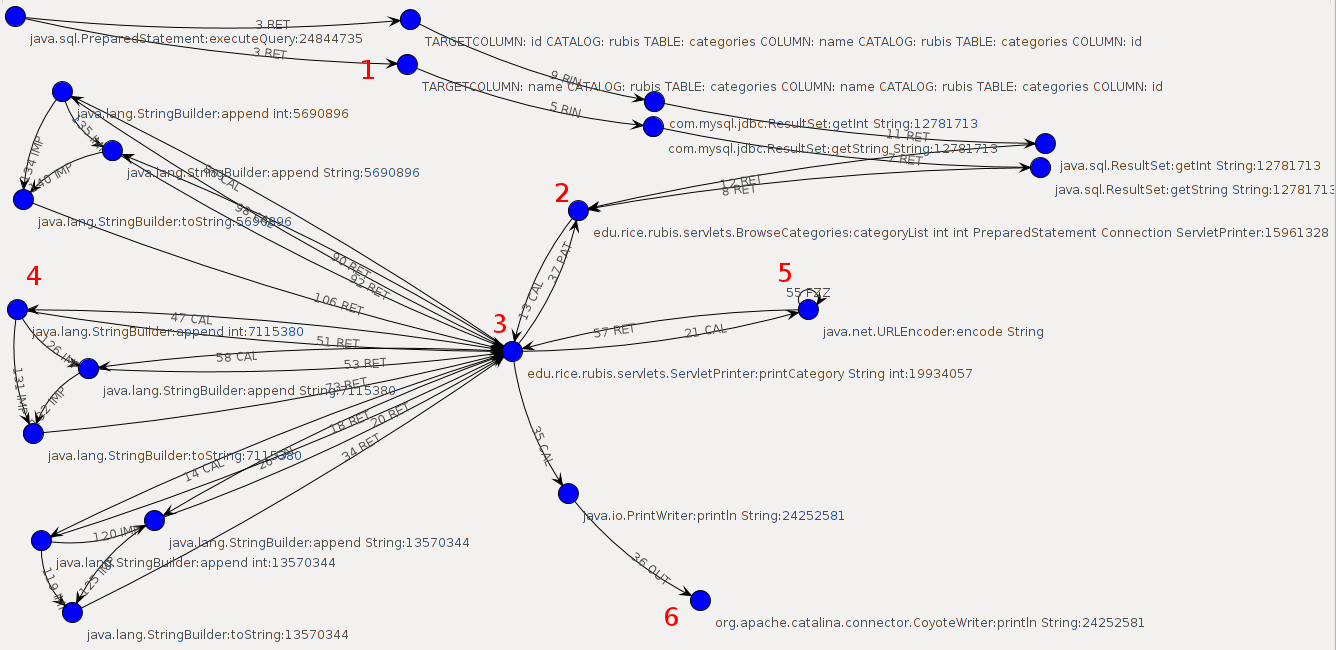
\includegraphics[width=1.0\textwidth]{figs/rubis_BrowseCategories_Numbered.eps}
    \caption[RUBiS Browse Categories Trace]{\label{fig:browsecategories} RUBiS Browse Categories Trace.}
  \end{center}
\end{figure}

\begin{sidewaysfigure}
\centering
\scalebox{0.43}
{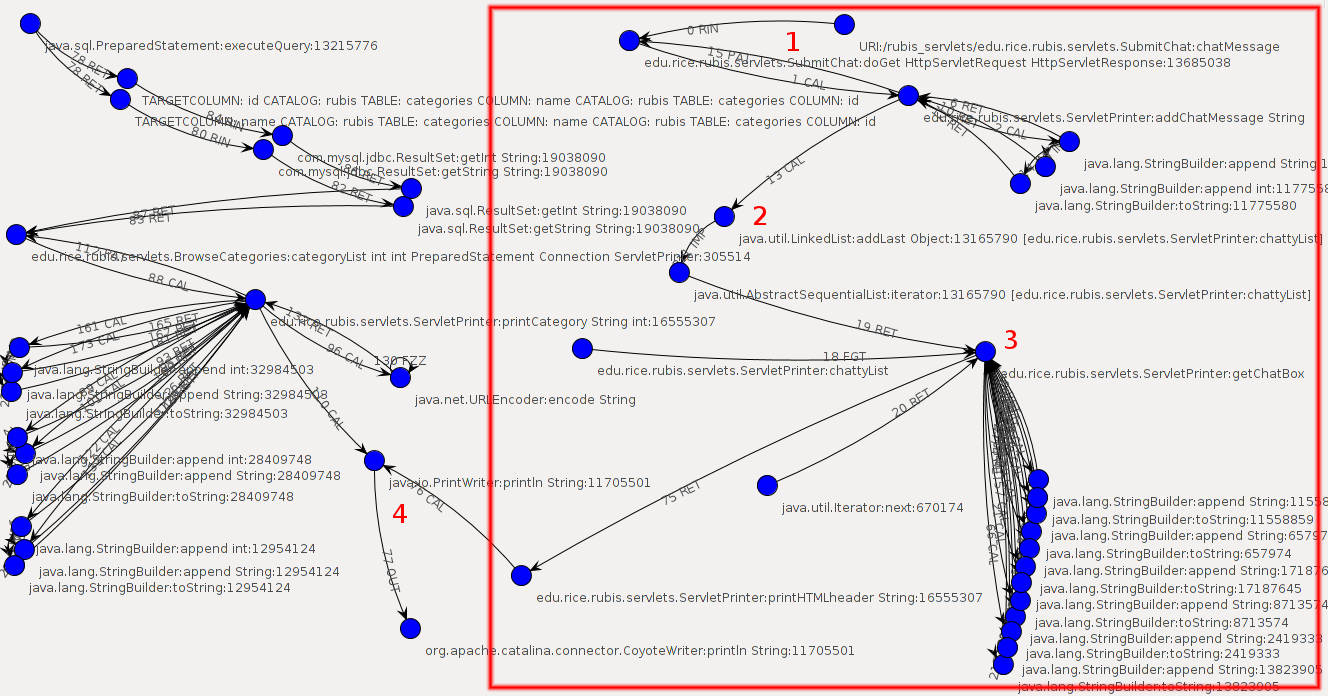
\includegraphics{figs/rubis_BrowseCategories_Chat_Numbered.eps}}
\caption{RUBiS Browse Categories With Chat Trace} 
\label{fig:browsecategorieschat}
\end{sidewaysfigure}

\begin{figure}[ht]
  \begin{center}
    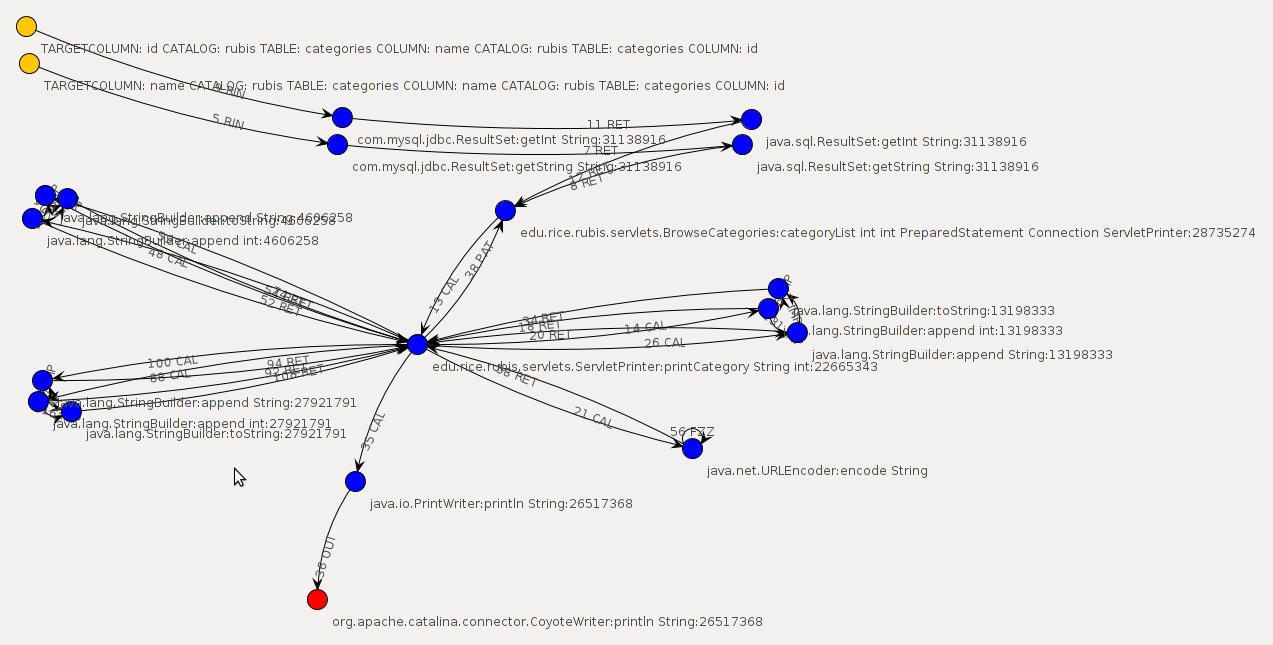
\includegraphics[width=1.0\textwidth]{figs/rubis_BrowseCategories_Precomp.eps}
    \caption[RUBiS Browse Categories Precomputation Results]{\label{fig:browsecategoriesprecomp} RUBiS Browse Categories Precomputation Results.}
  \end{center}
\end{figure}

\begin{figure}[ht]
  \begin{center}
    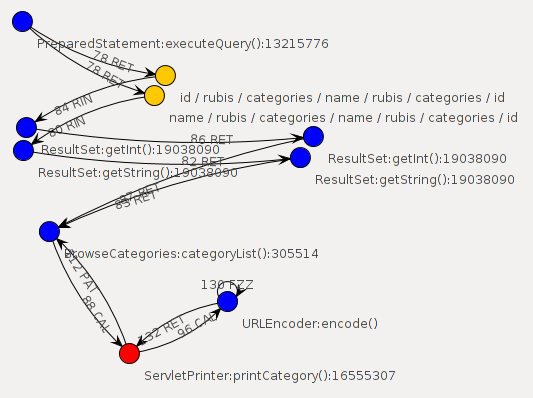
\includegraphics[width=1.0\textwidth]{figs/rubis_BrowseCategories_Chat_Precomp.eps}
    \caption[RUBiS Browse Categories With Chat Precomputation Results]{\label{fig:browsecategorieschatprecomp} RUBiS Browse Categories With Chat Precomputation Results.}
  \end{center}
\end{figure}

%\begin{figure}[ht]
%  \caption{\label{fig:outputBrowseCat} RUBiS Browse Categories Tainted Output.}
%\begin{verbatim}
%
%\end{verbatim}
%\end{figure}

%MAKE FIGURE:
%REQ: 1 - /rubis_servlets/edu.rice.rubis.servlets.BrowseCategories
%<title>RUBiS available categories</title> [NONTAINTED]
%<div style="border:solid 1px black;"><p>Popular Items</p> [NONTAINTED]
%<div style="border:solid 1px black;"><p>Chats</p></div><form action="/rubis_servlets/edu.rice.rubis.servlets.SubmitChat" method=POST> <input type=text size=20 name=chatMessage /> <input type=submit value="Post" /></form> [NONTAINTED]
%<h2>Currently available categories</h2><br> [NONTAINTED]
%<a href="edu.rice.rubis.servlets.SearchItemsByCategory?category=1&categoryName=Antiques+%26+Art+">Antiques & Art </a><br> [TAINTED: 20090212:id:2,20090212:name:1 [15759798] - TARGETCOLUMN: id CATALOG: rubis TABLE: categories COLUMN: name CATALOG: rubis TABLE: categories COLUMN: id #RECSEP#TARGETCOLUMN: name CATALOG: rubis TABLE: categories COLUMN: name CATALOG: rubis TABLE: categories COLUMN: id ]
%START: class org.apache.catalina.connector.CoyoteWriter END [NONTAINTED]
%<a href="edu.rice.rubis.servlets.SearchItemsByCategory?category=2&categoryName=Books+">Books </a><br> [TAINTED: 20090212:id:4,20090212:name:3 [15134979] - TARGETCOLUMN: id CATALOG: rubis TABLE: categories COLUMN: name CATALOG: rubis TABLE: categories COLUMN: id #RECSEP#TARGETCOLUMN: name CATALOG: rubis TABLE: categories COLUMN: name CATALOG: rubis TABLE: categories COLUMN: id ]
%START: class org.apache.catalina.connector.CoyoteWriter END [NONTAINTED]
%<a href="edu.rice.rubis.servlets.SearchItemsByCategory?category=3&categoryName=Business%2C+Office+%26+Industrial+">Business, Office & Industrial </a><br> [TAINTED: 20090212:name:5,20090212:id:6 [5433945] - TARGETCOLUMN: name CATALOG: rubis TABLE: categories COLUMN: name CATALOG: rubis TABLE: categories COLUMN: id #RECSEP#TARGETCOLUMN: id CATALOG: rubis TABLE: categories COLUMN: name CATALOG: rubis TABLE: categories COLUMN: id ]
%START: class org.apache.catalina.connector.CoyoteWriter END [NONTAINTED]
%<br><hr>RUBiS (C) Rice University/INRIA<br><i>Page generated by BrowseCategories in      8 seconds 518 milliseconds </i><br> [NONTAINTED]
%</body> [NONTAINTED]
%</html> [NONTAINTED]
%END MAKE FIGURE

%\begin{figure}[ht]
%  \caption{\label{fig:rubisPrecompDetails} RUBiS Precomputation Details.}
%\begin{verbatim}
%
%\end{verbatim}
%\end{figure}

%MAKE FIGURE
%Output Data:
%Node: org.apache.catalina.connector.CoyoteWriter:println String:26517368
%	Data: <a href="edu.rice.rubis.servlets.SearchItemsByCategory?category=1&categoryName=Antiques+%26+Art+">Antiques & Art </a><br>
%	Data: <a href="edu.rice.rubis.servlets.SearchItemsByCategory?category=2&categoryName=Books+">Books </a><br>
%	Data: <a href="edu.rice.rubis.servlets.SearchItemsByCategory?category=3&categoryName=Business%2C+Office+%26+Industrial+">Business, Office & Industrial </a><br>
%END MAKE FIGURE

%\begin{figure}[ht]
%  \caption{\label{fig:outputBrowseCatB} RUBiS Browse Categories With Chat Tainted Output.}
%\begin{verbatim}
%
%\end{verbatim}
%\end{figure}

%MAKE FIGURE:
%REQ: 3 - /rubis_servlets/edu.rice.rubis.servlets.BrowseCategories
%<title>RUBiS available categories</title> [NONTAINTED]
%<div style="border:solid 1px black;"><p>Popular Items</p> [NONTAINTED]
%<div style="border:solid 1px black;"><p>Chats</p><p>hello 1</p></div><form action="/rubis_servlets/edu.rice.rubis.servlets.SubmitChat" method=POST> <input type=text size=20 name=chatMessage /> <input type=submit value="Post" /></form> [TAINTED: 33440105:0 [12767107] - URI:/rubis_servlets/edu.rice.rubis.servlets.SubmitChat:chatMessage]
%<h2>Currently available categories</h2><br> [NONTAINTED]
%<a href="edu.rice.rubis.servlets.SearchItemsByCategory?category=1&categoryName=Antiques+%26+Art+">Antiques & Art </a><br> [TAINTED: 24037827:id:3,24037827:name:2 [640451] - TARGETCOLUMN: id CATALOG: rubis TABLE: categories COLUMN: name CATALOG: rubis TABLE: categories COLUMN: id #RECSEP#TARGETCOLUMN: name CATALOG: rubis TABLE: categories COLUMN: name CATALOG: rubis TABLE: categories COLUMN: id ]
%<a href="edu.rice.rubis.servlets.SearchItemsByCategory?category=2&categoryName=Books+">Books </a><br> [TAINTED: 24037827:id:5,24037827:name:4 [13477454] - TARGETCOLUMN: id CATALOG: rubis TABLE: categories COLUMN: name CATALOG: rubis TABLE: categories COLUMN: id #RECSEP#TARGETCOLUMN: name CATALOG: rubis TABLE: categories COLUMN: name CATALOG: rubis TABLE: categories COLUMN: id ]
%<a href="edu.rice.rubis.servlets.SearchItemsByCategory?category=3&categoryName=Business%2C+Office+%26+Industrial+">Business, Office & Industrial </a><br> [TAINTED: 24037827:name:6,24037827:id:7 [5340732] - TARGETCOLUMN: name CATALOG: rubis TABLE: categories COLUMN: name CATALOG: rubis TABLE: categories COLUMN: id #RECSEP#TARGETCOLUMN: id CATALOG: rubis TABLE: categories COLUMN: name CATALOG: rubis TABLE: categories COLUMN: id ]
%<br><hr>RUBiS (C) Rice University/INRIA<br><i>Page generated by BrowseCategories in      3 seconds 772 milliseconds </i><br> [NONTAINTED]
%</body> [NONTAINTED]
%</html> [NONTAINTED]
%END MAKE FIGURE

%\begin{figure}[ht]
%  \caption{\label{fig:rubisPrecompDetailsB} RUBiS Not Sure Figure.}
%\begin{verbatim}
%
%\end{verbatim}
%\end{figure}

%MAKE FIGURE
%Output Data:
%Node: edu.rice.rubis.servlets.ServletPrinter:printCategory String int:19112841
%	Data: <a href="edu.rice.rubis.servlets.SearchItemsByCategory?category=1&categoryName=Antiques+%26+Art+">Antiques & Art </a><br>
%	Data: <a href="edu.rice.rubis.servlets.SearchItemsByCategory?category=2&categoryName=Books+">Books </a><br>
%	Data: <a href="edu.rice.rubis.servlets.SearchItemsByCategory?category=3&categoryName=Business%2C+Office+%26+Industrial+">Business, Office & Industrial </a><br>
%END MAKE FIGURE

Figure~\ref{fig:browsecategoriesprecomp} shows the results of running the precomputation analysis over the same trace depicted in Figure~\ref{fig:browsecategories}. The first thing to notice here is that it is the same graph. Such is not always the case for this analysis, but in this instance the input trace was simple enough that the  analysis identified the entire trace as being precomputable. Consider the request in question, which only needs to access the categories table to list the names and ids of the categories to the user. Both the name and id columns of this table have been manually marked as being stable. This means that one does not expect category names or ids to be unpredictable - the same values will be present in the table for extended periods of application use. Given this information about these values and the input trace, the precomputation analysis determined that the tainted data flowing in this graph was entirely stable data, and thus the output of the analysis is the entire graph with the inputs and outputs coloured orange and red respectively. Additional data is obtained by viewing the details of the analysis, which mainly shows tainted data sent to each output node in the output graph. For this graph, the output node's data shows the HTML for three hyperlinks as in Figure C1b, these being the categories presented to the user. 

\paragraph{}
Interpreting this, a developer can reasonably assume that for the request responsible for this trace, the computation which reads category names and ids from the database and displays them to the user in this hyperlink form can be precomputed. At no point does this computation seemingly make use of any unpredictable data in generating the category hyperlinks, and so one could alter the application to essentially immediately output the hardcoded hyperlinks instead of fetching the data from the database and formatting it. If and when the category data does happen to change, one would then have to update the precomputed data, but it is assumed that this would happen very rarely.

\paragraph{}
The analysis can be taken further in this case. The tracking code not only logs tainted output, but also creates logs for non-tainted output. Using these one can observe the mixing of tainted and non-tainted data as it is composed together in the output. Looking to Figure C1, generated in the analysis tool from the output logs, we can see that the only tainted output involved in the response web page is from the three hyperlinks identified in the precomputation analysis. The rest of the data is non-tainted, and for this application this equates to it being hardcoded. Given these analysis results a developer can decide to simply precompute the entire response for this category listing page, saving on database access and formatting computation. 

\paragraph{}
Going further, RUBiS was modified to display a chat box on every page, allowing anyone to post messages to the server for everyone to see. Whenever a message is submitted by a user, it is posted to a SubmitChat servlet which is responsible for adding the message to a list of messages. The important thing to note about this data is that it is very unpredictable. The list of messages can change at any time, with random data input to them, and as such any computations which work with this data are poor candidates for any kind of caching. Figure~\ref{fig:browsecategorieschat} shows a trace for the same page load as before, but including a post to the chat box. The left side of the graph in the figure is as before, the portion outlined in the red box shows the additional flow of the chat message data. This new portion of the graph actually spans two requests to the application - one to submit the chat message and another to display the list of categories along with the new message. The portion of the graph from labeled points 1 to 2 covers the submission of the message, starting with the source node showing the relative URI of the request and the name of the tainted parameter, 'chatMessage'. This parameter is accessed by the doGet method of the SubmitChat servlet, passed to the addChatMessage method of a ServletPrinter Object where it is concatenated with some formatting text, and finally appended to a LinkedList at point 2 by the addLast method. Note that the label for this addLast node ends in the name of a field, the 'chattyList' field of a ServletPrinter Object. This means that this field points to the LinkedList in question and indicates that by storing tainted data in the LinkedList it is effectively stored in that field. Such is useful for a developer to know when interpreting these graphs and mapping them back to the code responsible for them. Point 3 shows where the chat message data flows for the category list request, as a LinkedList is read from the chattyList along edge 18 in the getChatBox method. Following that an iterator over the LinkedList returned along edge 19, and the iterator is accessed along edge 20. The messages inside are concatenate with some formatting text before being passed along to point 4, being returned to the printHTMLHeader method of a ServletPrinter Object and written to the user response stream along with the list of categories.

\paragraph{}
Figure~\ref{fig:browsecategorieschatprecomp} shows the result of the precomputation analysis on the trace from Figure~\ref{fig:browsecategorieschat}. It is exactly like the analysis results from Figure~\ref{fig:browsecategoriesprecomp} except that the precomputation ends at the red PrintCategory node, no longer extending to the println nodes. This is because the println method on the same PrintWriter Object now also receives the random data of the chat messages, and thus one cannot replace calls to this method with precomputed data. Given the precomputation output in Figure C2b and the response output breakdown in Figure C2, a developer can determine that the page can be mostly precomputed, only needing to dynamically generate the portion tainted by the chatMessage data.

% The traces for jgossip will not really be shown and described in detail (at least not the pre-analysis traces), will be more about showing the post analysis trace and describing the implications of it
\subsubsection{jGossip} 

\begin{sidewaysfigure}
\centering
\scalebox{0.42}
{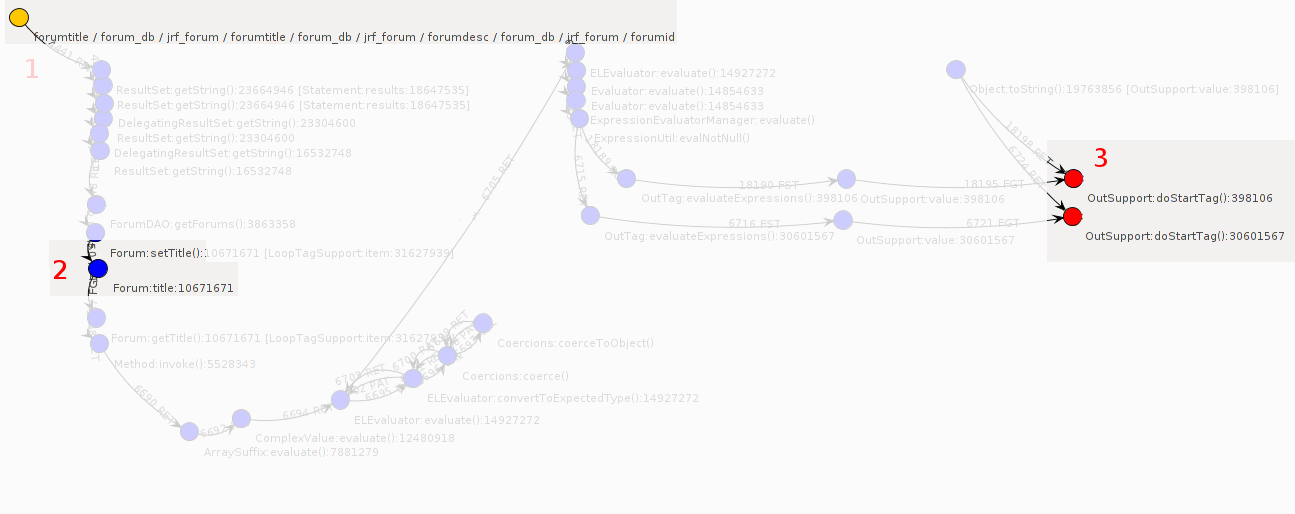
\includegraphics{figs/jgossip_MainPage_Precomp.eps}}
\caption{jGossip Main Page Precomputation Analysis Results} 
\label{fig:mainpageprecomp}
\end{sidewaysfigure}

\paragraph{}
Loading the main page of the jGossip application, which presents users with a list of available forums, and running the precomputation analysis over the dataflow produces the graph shown in Figure~\ref{fig:mainpageprecomp}. This graph is filtered to show the flow of a particular data item, the title of a forum displayed on the page.

\paragraph{}
The analysis essentially indicates that the data is able to flow from the database all the way to output without any dependence on other inputs, in particular inputs with unpredictable values. Breaking this flow down, the data read from the database at point 1, and eventually stored in a field near point 2. This field is subsequently accessed by JSP generated code at point 2 (Method:invoke() indicates the use of reflection to get to the field), and the forum title passes through a series of internal methods from the JSTL tab library (the 'evaluate' nodes). It is ultimately used in the doStartTag() method at point 4, a method used by JSP tags to write data to the user response page.

\paragraph{}
Using this result, along with others which show similar results for other flows of data on the main page, one can find large portions of the main page which can simply be precomputed and then updated should the input database tables ever change. The precomputed results could be added to the JSP pages, avoiding the entire computation which reads them from the database and invokes the JSTL library.

\subsection{Caching}
\subsubsection{RUBiS}

\begin{sidewaysfigure}
\centering
\scalebox{0.43}
{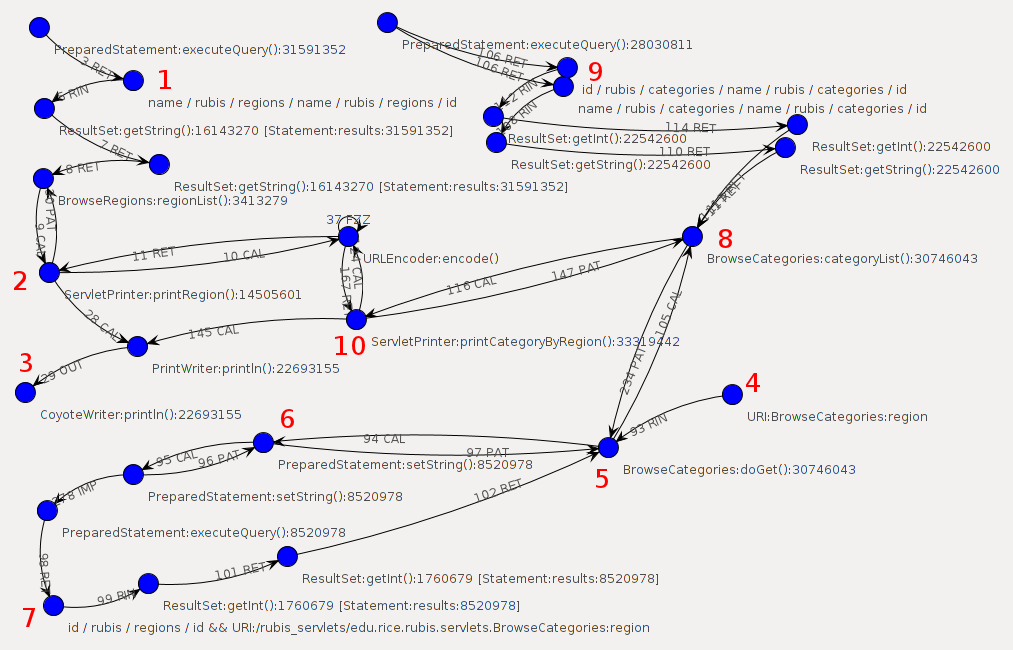
\includegraphics{figs/rubis_BrowseRegionCategories_Numbered.eps}}
\caption{RUBiS Browse Categories By Region Trace} 
\label{fig:browseregioncategories}
\end{sidewaysfigure}

\begin{sidewaysfigure}
\centering
\scalebox{0.41}
{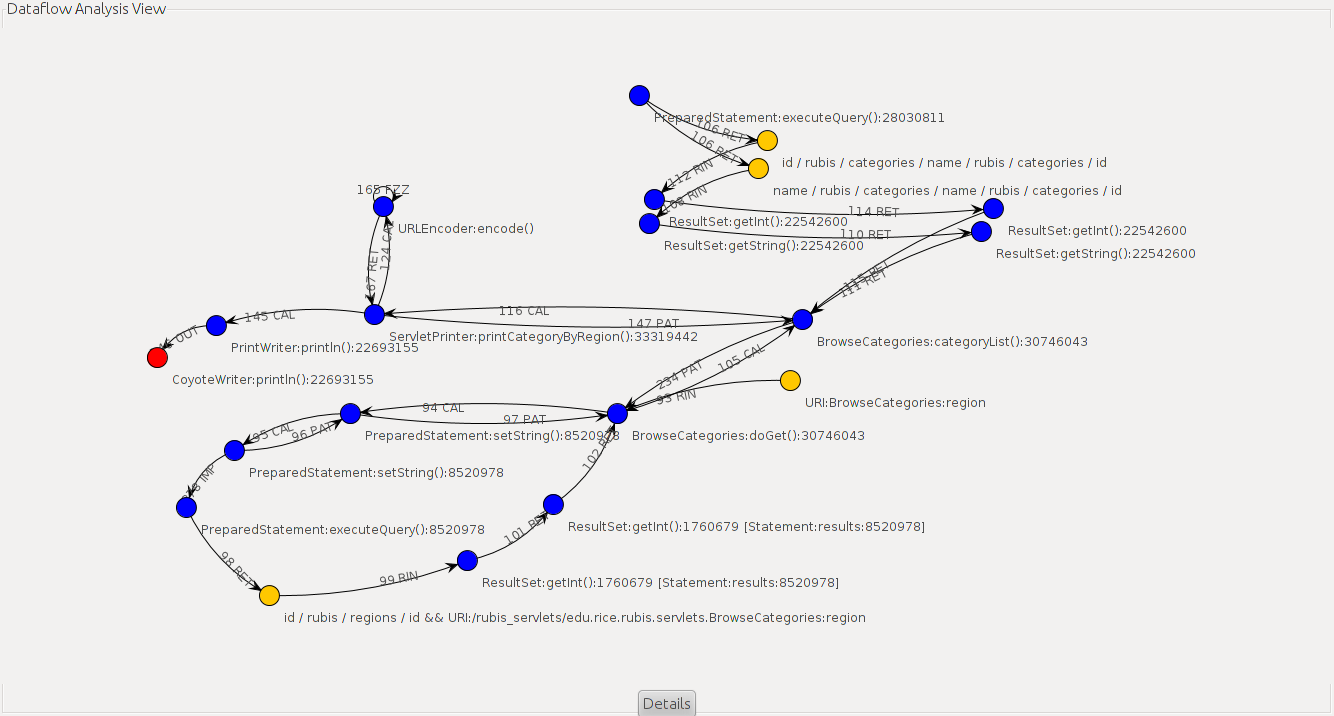
\includegraphics{figs/rubis_BrowseRegionCategories_Caching.eps}}
\caption{RUBiS Browse Categories By Region Caching Results} 
\label{fig:browseregioncategoriescaching}
\end{sidewaysfigure}

%MAKE FIGURE
%REQ: 3 - /rubis_servlets/edu.rice.rubis.servlets.BrowseCategories
%<title>RUBiS available categories</title> [NONTAINTED]
%<div style="border:solid 1px black;"><p>Popular Items</p> [NONTAINTED]
%<div style="border:solid 1px black;"><p>Chats</p></div><form action="/rubis_servlets/edu.rice.rubis.servlets.SubmitChat" method=POST> <input type=text size=20 name=chatMessage /> <input type=submit value="Post" /></form> [NONTAINTED]
%<h2>Currently available categories</h2><br> [NONTAINTED]
%<a href="edu.rice.rubis.servlets.SearchItemsByRegion?category=1&categoryName=Antiques+%26+Art+&region=1">Antiques & Art </a><br> [TAINTED: 30453968:id:6,3156700:name:8,3156700:id:9,23441609:4 [4724538] - TARGETCOLUMN: id CATALOG: rubis TABLE: regions COLUMN: id #RECSEP#TARGETCOLUMN: name CATALOG: rubis TABLE: categories COLUMN: name CATALOG: rubis TABLE: categories COLUMN: id #RECSEP#TARGETCOLUMN: id CATALOG: rubis TABLE: categories COLUMN: name CATALOG: rubis TABLE: categories COLUMN: id #RECSEP#URI:/rubis_servlets/edu.rice.rubis.servlets.BrowseCategories:region]
%<a href="edu.rice.rubis.servlets.SearchItemsByRegion?category=2&categoryName=Books+&region=1">Books </a><br> [TAINTED: 30453968:id:6,23441609:4,3156700:id:11,3156700:name:10 [575947] - TARGETCOLUMN: id CATALOG: rubis TABLE: regions COLUMN: id #RECSEP#URI:/rubis_servlets/edu.rice.rubis.servlets.BrowseCategories:region#RECSEP#TARGETCOLUMN: id CATALOG: rubis TABLE: categories COLUMN: name CATALOG: rubis TABLE: categories COLUMN: id #RECSEP#TARGETCOLUMN: name CATALOG: rubis TABLE: categories COLUMN: name CATALOG: rubis TABLE: categories COLUMN: id ]
%<a href="edu.rice.rubis.servlets.SearchItemsByRegion?category=3&categoryName=Business%2C+Office+%26+Industrial+&region=1">Business, Office & Industrial </a><br> [TAINTED: 30453968:id:6,23441609:4,3156700:name:12,3156700:id:13 [33336785] - TARGETCOLUMN: id CATALOG: rubis TABLE: regions COLUMN: id #RECSEP#URI:/rubis_servlets/edu.rice.rubis.servlets.BrowseCategories:region#RECSEP#TARGETCOLUMN: name CATALOG: rubis TABLE: categories COLUMN: name CATALOG: rubis TABLE: categories COLUMN: id #RECSEP#TARGETCOLUMN: id CATALOG: rubis TABLE: categories COLUMN: name CATALOG: rubis TABLE: categories COLUMN: id ]
%<br><hr>RUBiS (C) Rice University/INRIA<br><i>Page generated by BrowseCategories in      3 seconds 973 milliseconds </i><br> [NONTAINTED]
%</body> [NONTAINTED]
%</html> [NONTAINTED]
%END MAKE FIGURE

%MAKE FIGURE
%Output Data:
%Node: org.apache.catalina.connector.CoyoteWriter:println String:22693155
%	Data: <a href="edu.rice.rubis.servlets.BrowseCategories?region=AZ--Phoenix">AZ--Phoenix</a><br>
%	Data: <a href="edu.rice.rubis.servlets.BrowseCategories?region=CA--Los+Angeles">CA--Los Angeles</a><br>
%	Data: <a href="edu.rice.rubis.servlets.BrowseCategories?region=CA--Oakland">CA--Oakland</a><br>
%	Data: <a href="edu.rice.rubis.servlets.SearchItemsByRegion?category=1&categoryName=Antiques+%26+Art+&region=1">Antiques & Art </a><br>
%	Data: <a href="edu.rice.rubis.servlets.SearchItemsByRegion?category=2&categoryName=Books+&region=1">Books </a><br>
%	Data: <a href="edu.rice.rubis.servlets.SearchItemsByRegion?category=3&categoryName=Business%2C+Office+%26+Industrial+&region=1">Business, Office & Industrial </a><br>
%END MAKE FIGURE

\paragraph{}
Figure~\ref{fig:browseregioncategories} shows a trace taken from viewing the same RUBiS categories list as previously shown with an additional constraint. For this trace, a user first submits a request to get a list of geographical regions. Once these are displayed, a user picks a region, which submits another request to obtain the category list. The region name selected in the first request is used to obtain a region id, which is included in the category hyperlinks output to the user in the second request. The important point to note is that this category list should not be outright precomputed, as the region id parameter varies based on user input. However, this region id is over a small enough range that it is reasonably predictable, and thus it seems that a cache could be implemented here. Breaking down Figure~\ref{fig:browseregioncategories}, point 1 shows the region name data being read from the database for the first request. Note that this trace has been filtered to hide string concatenation dataflow (removing StringBuilder nodes), make it more presentable. At point the region names are passed to the encode method during concatenation with formatting text, and then output to the user at point 3. A user clicks on a region, submitting its name as a parameter in the next request. This is shown at point 4, as the 'region' parameter. From point 5 along to point 6 and continuing, the region name is set as a parameter on a PreparedStatement Object to be used as a predicate in a database query. When the query is executed at point 7, note how the input node is labeled as being tainted by not only the id column from the regions table, but also by the region parameter that the query was predicated on. Point 5 receives the region id, and passes it to point 8, which receives category names and ids from point 9. The category data and region id are sent point 10, the 'printCategoryByRegion' method, which concatenates them with formatting text, encodes them, and writes them out to the user at point 3.

\paragraph{}
Running the caching analysis over this graph and filtering the results to only show the dataflow for the second request, the result graph show in Figure~\ref{fig:browseregioncategoriescaching} is obtained. The first important point to note is that this graph was not eligible for precomputation, due to the influence of the user-supplied region parameter in every part of this graph except for the upper-left portion showing the flow of the category name/id data. However, since this parameter has been marked as being predictable (see Figure Ce [datasourceinfochart]), the analysis judges that a cache may be possible for the identified inputs. Interpreting this, a developer can start at the output node. Figure Cf shows the tainted data flowing here, and this can be compared to the response output breakdown shown in Figure Cg. Evidently the entire page it composed non-tainted (likely static) data and the cachable output. Looking at the inputs in the graph, the data responsible for the cachable output comes from database tables which have all been marked as stable, unlikely to change frequently, and the predictable region parameter. 

\paragraph{}
Using the graph and some rudimentary knowledge of the application, a cache could be implemented as follows. First, consider the inputs. All of them, save for the region parameter, are stable, and thus the only parameter the cache need use to store and return results is that region parameter. For the other inputs, like those from the categories and regions tables, these data sources need only to be monitored to detect if they are modified. If so, the cached results are invalidated to be regenerated. As the doGet node is the first to receive the region parameter, the cache check could be performed there. If the cache hits for a given region, the output data (perhaps the entire response page or just the category hyperlinks) can be returned and written to the response stream. In the event of a cache miss, the computation can proceed as normal, and the results picked up in the printCategoryByRegion node to be placed in the cache for later.

\subsubsection{jGossip} 

\begin{sidewaysfigure}
\centering
\scalebox{0.44}
{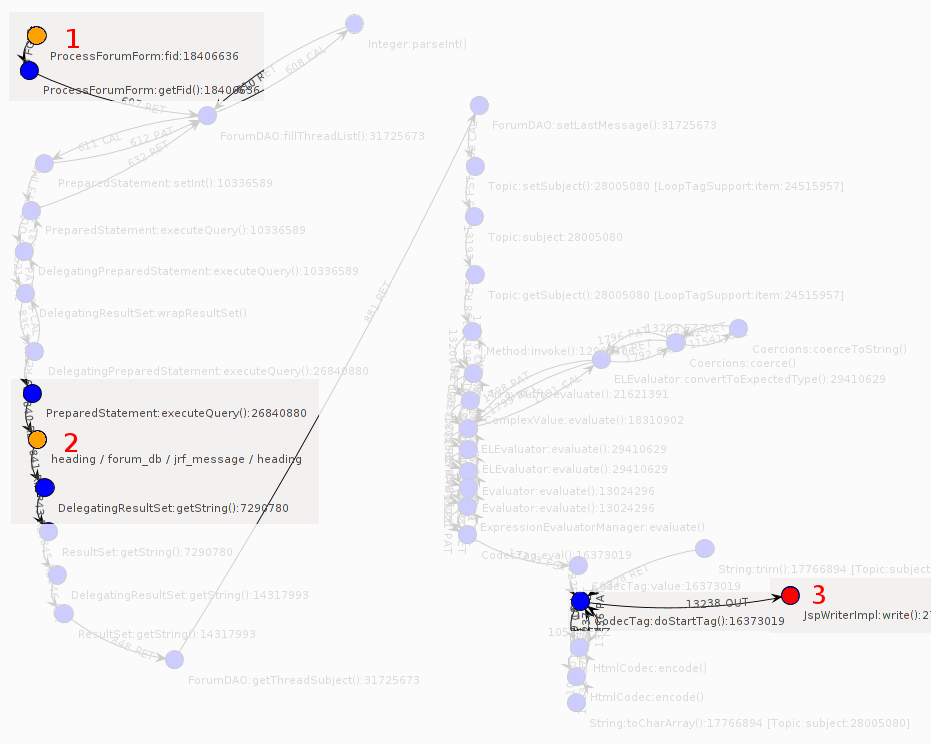
\includegraphics{figs/jgossip_ViewForums_Caching.eps}}
\caption{jGossip View Forums Caching Results} 
\label{fig:viewforumscaching}
\end{sidewaysfigure}

The caching analysis for jGossip is significantly more difficult due to the much larger traces produced by the application. This is caused by libraries, like JSTL, used by jGossip, and typically the traces were around 40K communication events for handling a single request (whereas RUBiS had around 400). This presented some very large, complex graphs, which would not be amenable to a manual analysis, and which were still challenging to assess automatically. Nevertheless, Figure~\ref{fig:viewforumscaching} shows a graph obtained from the analysis tool which indicates the existence of a possible cache.

\paragraph{}
This was obtained by tracing the application while selecting a forum from the application's main menu, which then displayed a page giving some information about the forum including a message from it. The trace shows how the forum id (fid) supplied by the user when selecting a forum (point 1) acts as the sole input to a database query which fetches a message heading from the database (point 2). This heading is then passed through a series of methods, ultimately being output to the response page at point 3. The fact that this path was identified by the analysis means that the data which flows along the path is not influenced by random input. We can see how given a fid value, of which there are a limited set, and knowing whether or not the messages in that forum have been updated, we can either return a cached message heading or generate one to fill the cache.

\paragraph{}
Given this graph, it is up to the developer to investigate the feasibility of this cache. The analysis data can additionally provide stack traces to identify the control flow responsible for each communication event, to help in choosing where to implement any changes.

\subsection{Postcomputation}
\subsubsection{RUBiS}

\begin{sidewaysfigure}
\centering
\scalebox{0.44}
{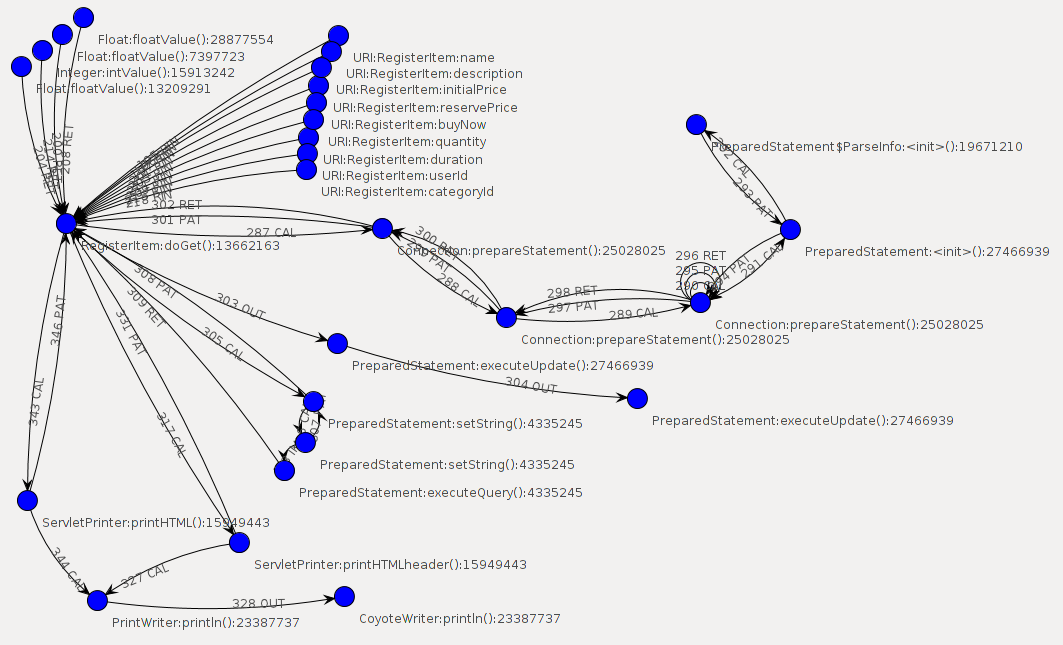
\includegraphics{figs/rubis_SellItem_Numbered.eps}}
\caption{RUBiS Sell Item Trace} 
\label{fig:sellitemtrace}
\end{sidewaysfigure}

\begin{sidewaysfigure}
\centering
\scalebox{0.44}
{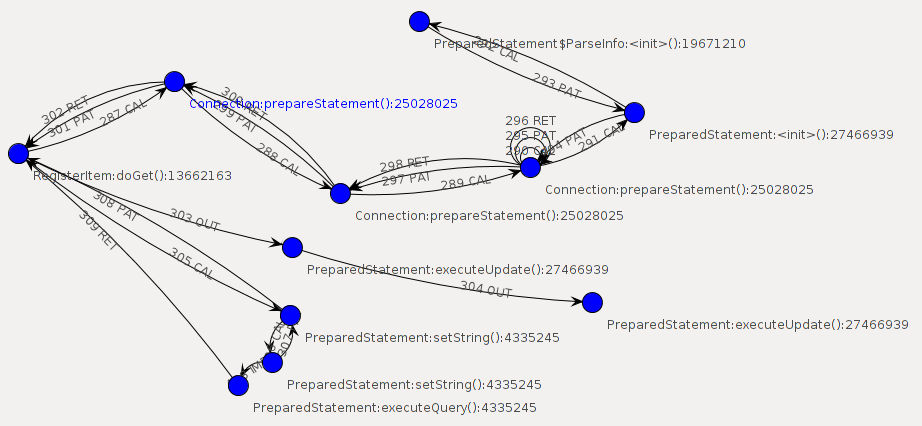
\includegraphics{figs/rubis_SellItem_PostComp.eps}}
\caption{RUBiS Sell Item Postcomputation Analysis Results} 
\label{fig:sellitempostcomputation}
\end{sidewaysfigure}

For the postcomputation analysis, we sell an item on the RUBiS Store. This simply involves filling out a web form describing various details of the item (name, price, etc), and submitting this to a RegisterItem servlet. The item is added to the database and the item details are displayed back to the user. 

\paragraph{}
The dataflow for this is given in Figure~\ref{fig:sellitemtrace}. At point 1 the various parameters describing the item are read, and some of them are converted to numeric values at point 2 (and hence tracked by the numeric tracking system). The RegisterItem:doGet() method then uses these parameters to construct a PreparedStatement at point 3, which is to execute a database update at point 4. This is the update which inserts the item into the database. Following this, some of the parameters are used at point 5 to query the database checking if the item was inserted. Finally, at point 6, the parameters are written back to the response page.

\paragraph{}
Figure~\ref{fig:sellitempostcomputation} shows the results of the postcomputation analysis over this graph. What this indicates is parts of the dataflow which could be delayed until later, namely the database update/query flows at points 3, 4, and 5 from Figure~\ref{fig:sellitemtrace}. Missing from this graph is the reading of the item properties and writing them to the response page. This is because if these flows were deferred until later the output that the user sees would be incomplete. The analysis reveals that the database queries return no data which goes to the user response, and thus the analysis suggests that these queries could be done asynchronously, returning back to the user without waiting for their completion.

\subsubsection{jGossip} 

A caching analysis for jGossip was significantly more difficult due to the greater complexity of the traces produced. This was largely due to the use of such external libraries as JSTL which jGossip relies on to format its output, producing traces of over 40K communication events for simple application actions vs around 300 for RUBiS. Nevertheless, the analysis tool was successfully used to capture the existence of a caching opportunity in jGossip.

\begin{sidewaysfigure}
\centering
\scalebox{0.5}
{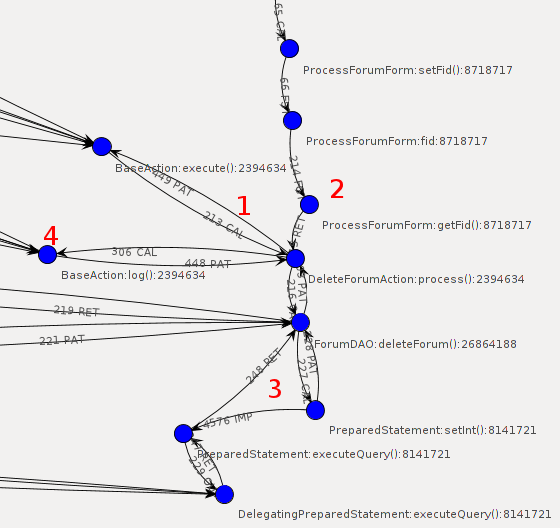
\includegraphics{figs/jgossip_DeleteForum_PostComp.eps}}
\caption{jGossip Delete Forum Postcomputation Analysis Results} 
\label{fig:deleteforumpostcomputation}
\end{sidewaysfigure}

\paragraph{}
To test the postcomputation analysis for jGossip, we use a trace taken while deleting a forum. We anticipated that this action would involve computation and updates to the database which could potentially be deferred, being separate from any computation responsible for displaying output to the user.

\paragraph{}
Figure~\ref{fig:deleteforumpostcomputation} shows a partial view of the results of the analysis. At point 1 an object containing data to service the request, such as the ID of the forum to delete, is passed into an Action object (Actions basically provide the entry point functionality in an Apache struts application, like the servlets used in RUBiS). Point 2 shows the accessing of the forum ID from the data object. This ID is passed to the highlighted deleteForum() method, which in turn uses it in a query which deletes the forum from the database. Finally, at point 4 we see that not only can the process which deletes the forum be deferred, but also a logging action. The analysis is showing that the path of data presented in Figure~\ref{fig:deleteforumpostcomputation} likely does not reach any output necessary to generate the user response page. At this point it is up to the developer to inspect this path and determine if they wish to make elements of it occur asynchronously to speed the response to the user.

\subsection{Persistent State}
\subsubsection{RUBiS}

\begin{sidewaysfigure}
\centering
\scalebox{0.5}
{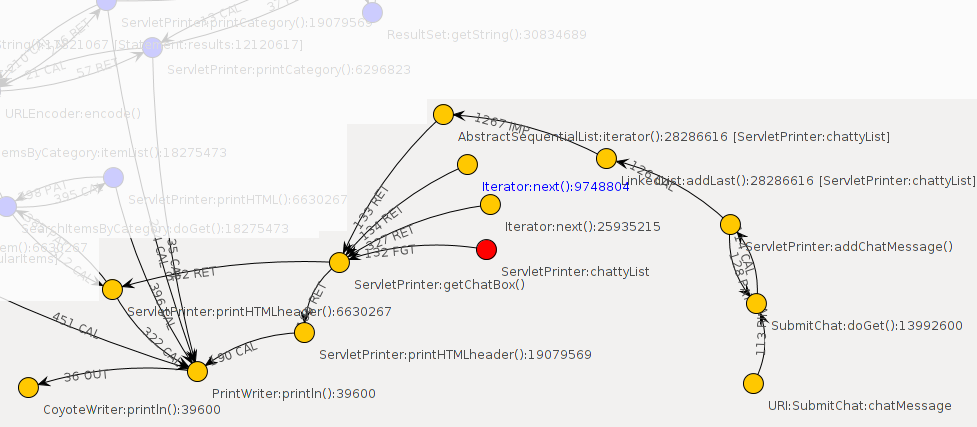
\includegraphics{figs/rubis_BrowseItems_State.eps}}
\caption{RUBiS Browse Items State Analysis Results} 
\label{fig:browseitemsstate}
\end{sidewaysfigure}

Figure~\ref{fig:browseitemsstate} shows the location of persistent state when interacting with the RUBiS chat box, as previously described in section~\ref{sec:rubisprecomp}. Only the portion of the graph which deals with the persistent state is shown here. The red node shows where the persistent state is actually kept, in a variable called 'chattyList' on the ServletPrinter class. The orange nodes indicate any nodes which communicated the persistent data in question. As expected, these  orange nodes include a chatMessage parameter and its flow into the chattyList, as well as the output nodes which indicate the writing of the chat messages out to the user.

\paragraph{}
Other instances of persistent state existed in the application, in static variables like this one. All of these were known prior to the automated analysis, which was able to identify them easily.

\subsubsection{jGossip} 

This analysis revealed several instances of persistent state in the jGossip application, mainly session attributes storing data read from the database for quick lookup, such as forum threads and messages. We do not present the results here, as the analysis is a basic one and explored sufficiently in the RUBiS example. Furthermore, the next analysis, user state, subsumes this one and deals with the jGossip application.

\subsection{User State}
\subsubsection{RUBiS}

The RUBiS application did not contain any persistent state which was not shared between multiple users, mainly due to the fact that it had no notion of sessions.

\subsubsection{jGossip}

\begin{sidewaysfigure}
\centering
\scalebox{0.44}
{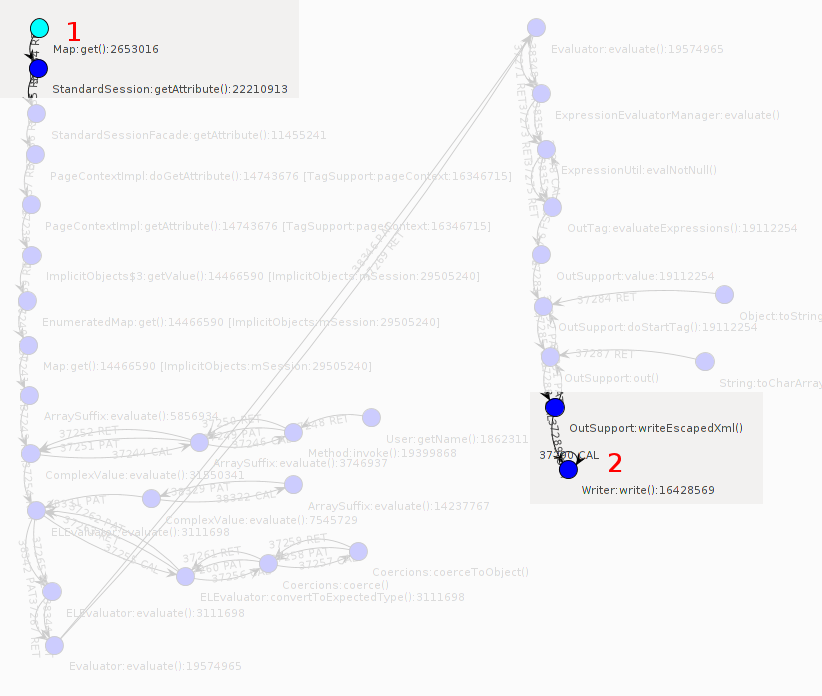
\includegraphics{figs/jgossip_BiLogin_UserState.eps}}
\caption{jGossip Login User State Analysis Results} 
\label{fig:loginstate}
\end{sidewaysfigure}

For this analysis we traced jGossip while logging in with two different users, each coming from a different IP address. This was done in order to generate persistent state data which potentially would be only shared with a single user. We ran the automated user state analysis, and identified the flow show in Figure~\ref{fig:loginstate}. Though it is not readily apparent in the figure, the analysis tool additionally mapped the tainted data in the flow to user response output, revealing that this data is a user name used to populate a username field which appears on every page.

\paragraph{}
The fact that the analysis identified this flow indicates that this username data has been used over multiple requests, but is only ever shared with a single user. At point 1 in the figure we can see where the data is stored, in a Java Map object, which is the underlying implementation for the Session objects on which getAttribute is called as one follows the flow. The data proceeds through a series of evaluate methods, which are a result of using JSP and JSTL, before being output at point 2.

\paragraph{}
Knowing that this data is only shared with a single user, one could potentially remove this logic from the server-side code and allow the client to store their own username. The flow shown gives a developer some clues about what the implications of this would be, in that they may need to emulate some of the operations that the JSTL code performed in order to properly display the data to the user. This amounts to relocating the path shown in the figure from the server to the client, starting with moving the data (point 1), then the computation, and finally outputting it to the user (point 2).

\subsection{Wasteful Communication}
\subsubsection{RUBiS}

The RUBiS application did not exhibit significant wasteful communication, due to its simple design.

\subsubsection{jGossip} 

\begin{sidewaysfigure}
\centering
\scalebox{0.2}
{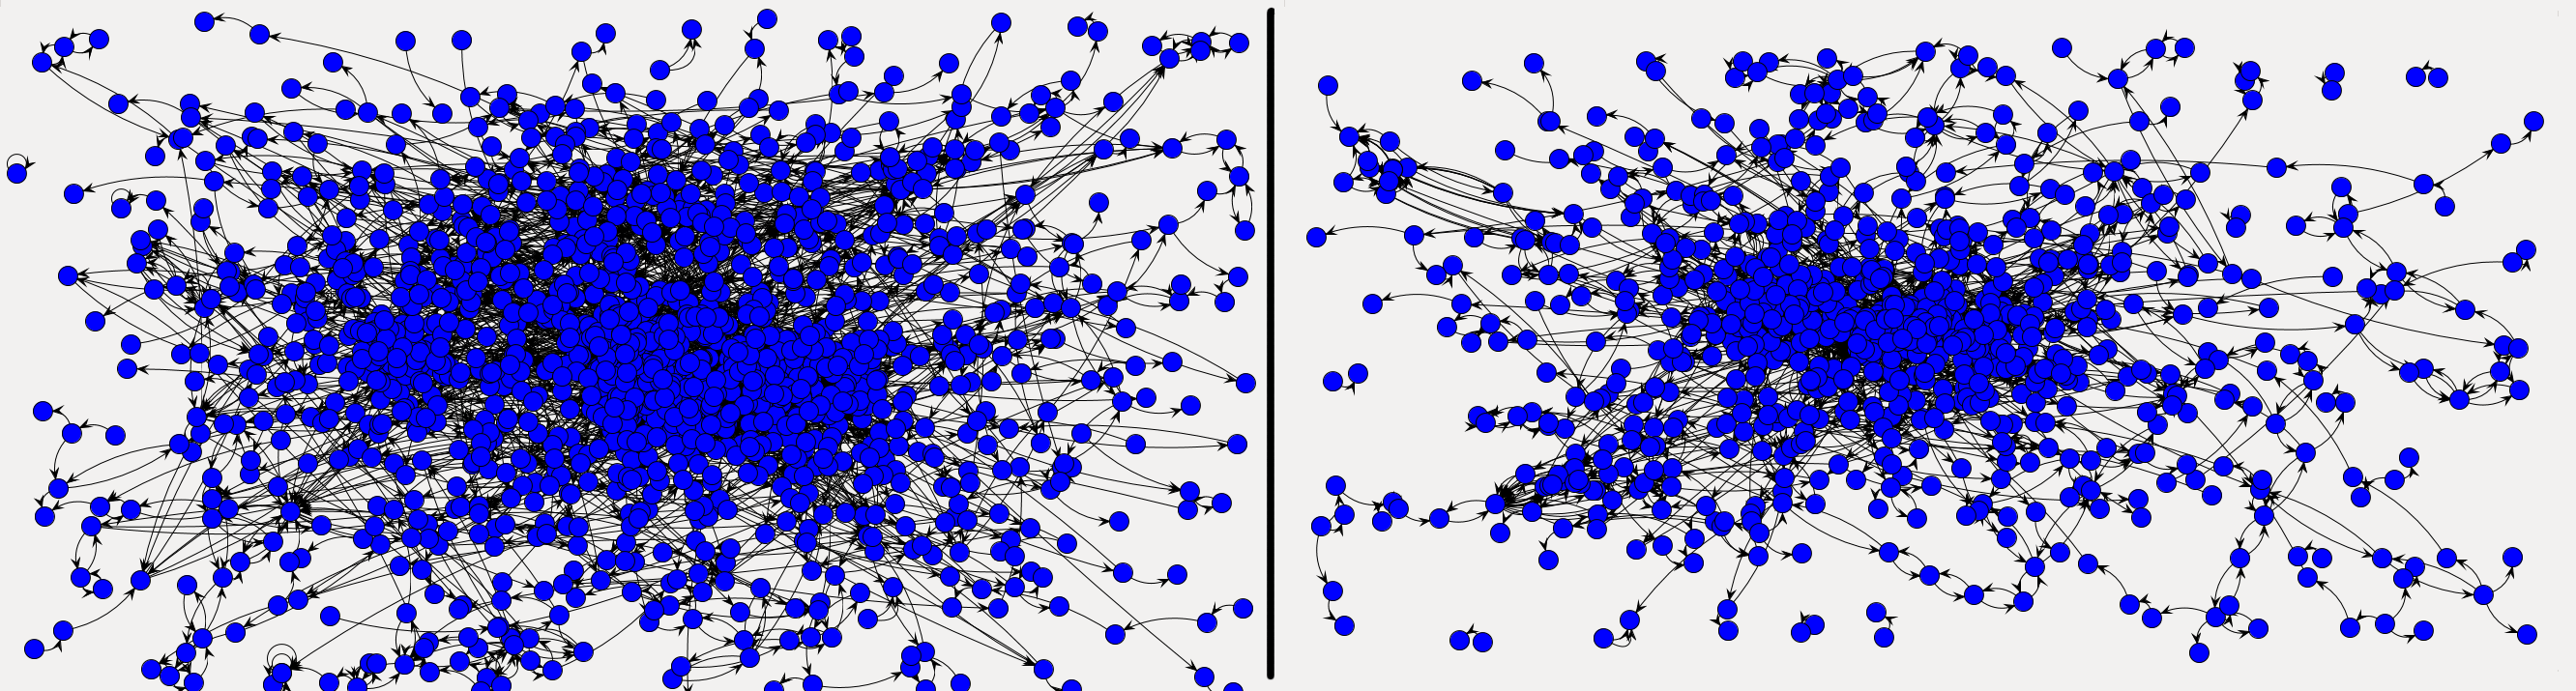
\includegraphics{figs/jgossip_ShowForum_WasteComm.eps}}
\caption{jGossip Wasteful Communication Analysis Results} 
\label{fig:showforumcomm}
\end{sidewaysfigure}

This analysis was a very simple one, and serves to hint at the potential for this technique. Figure~\ref{fig:showforumcomm} shows views of the same trace. On the left is shown every instance where tainted data is communicated when the users requests to view a forum (the same trace used in the caching analysis). On the right we have removed every edge which carries tainted data which is never actually used, resulting in a significantly smaller graph (5921 of the original 14693 edges remained).

\paragraph{}
In jGossip this is largely due to the use of JSP, which passes around objects containing references to all the data needed to render a page, whether or not they are needed in a particular function. The figure serves to show that such an occurence can be quite prevalent in certain applications, and that our analysis tool is capable of detecting it.

\chapter{Conclusions} % DIFFICULT

\section{Discussion of Results}

Having run most of the analyses over both applications, identifying the analysis targets from the taint trace data using the automated tool, the experiments were largely successful. In particular, the results for the precomputation analysis on both applications were impressive. In both cases the analysis was able to proceed with minimal user intervention to produce the graphs presented here. All that was needed was the initial input source descriptions files, as well as some manual filtering out of nodes for some of the jGossip graphs for presentation purposes.

\paragraph{}
The caching analysis, especially on the RUBiS application, was able to not only identify the existence of cachable output, but also show in a clean manner all the inputs to consider for the cache. For RUBiS, one can easily see how the various inputs from both the user and database come together to determine the result, and thus a developer should be able easily use this in implementing a cache for the data in question. It is useful to see the path of all the relevant data, quickly indicating the computations responsible for transforming it to what the user sees. Additionally, the small graph sizes for RUBiS means that the analysis results are easy for one to grasp immediately once presented by the tool. 

\paragraph{}
Also impressive was the user state analysis for jGossip. Looking for dataflow paths present in multiple requests but not shared with more than one user produced some very clean graphs, like the one shown. It was easy to identify the location of the persistent data, and then subsequently the sequence of communications and computations needed to take the data to its destination. However, not all of the graphs produced by the analyses were so clean.

\paragraph{}
In the case of jGossip, the much larger graph sizes meant that more intervention was needed to obtain the presented results. The caching analysis for jGossip identified tainted dataflow graphs which were cachable, only involving the flow of predictable data. However, they were too large to immediately grasp, containing large groups of nodes from calls into frameworks which ultimately distracted from the dataflows which would most likely be interesting to a developer. The graph shown was obtained by inspecting some of the jGossip source to understand how the cachable data was likely flowing, and then searching in the analysis results for the occurence of this. Following that, nodes which did not contribute to the interesting dataflow were manually filtered out.

\paragraph{}
Heavier manual intervention was also needed for the jGossip post computation analysis, where again some knowledge of the code and what we expected the analysis to actually find helped to locate the results in the large output graphs. For post computation, there were many nodes in jGossip which carried tainted data which never made it to the user, and as such were identified by the analysis. Since we wanted to focus on just the nodes which contributed to a deferable database write, some filtering was needed to present the graph.

\paragraph{}
This brings us to the point of the difficulty of automating these kinds of analyses. Our results with the RUBiS application were very optimistic, as the graphs produced by the analysis tool were very easy to understand immediately in large part thanks to their small size. Additionally, since RUBiS uses no added libraries, every node in the graph is potentially relevant to the developer and amenable to change and optimization under the guidance of the analysis.

\paragraph{}
For a framework-heavy application like jGossip, and realistically many Java web applications make extensive use of large frameworks, the graphs are much larger. At their current stage, most of our analyses output results which are negatively affected by this complexity. They suffer from a "rats nest" effect, and require some manual filtering and searching through to find the parts which could be used to actually support a developer in optimizing the applicaiton. The results are still there, they are just surrounded in many nodes which are less relevant, and thus it helps at this point to actually know what you are looking for. Even knowing simply which piece of data may be involved in an optimizating can go a long way. For the jGossip caching analysis the output was greatly simplified by using the tool to focus on nodes which carried data which we suspected would be cachable.

\paragraph{}
A related problem, again most prevalent in the large jGossip graphs, is that of false positives. The analyses are written to be fairly general, so as to find their results in applications which were not written to be easily analyzed. Every pattern of dataflow cannot be reasonably anticipated, so the analyses were written to be permissive and present many possible results. From these one can find those which are truly useful. For example, in the caching analysis for jGossip it was possible for some some output to be affected by random data through control dependence, which our taint tracking technique does not consider.

\paragraph{}
A final problem, unrelated to the analysis results, is that of the speed of applications during taint tracking. Slowdowns of roughly two orders of magnitude were observed, especially in the more complex jGossip application. This is mainly because of the use of AspectJ, which introduced inefficiencies inherent in its own design as well as forced us to perform some wasteful workarounds to properly track tainted data. This reality, along with the fact that the log files could be very massive for even small amounts of application activity (10s of thousands of lines per request in jGossip), meant that we generally did not perform analyses over exhaustive taint traces. By this we mean that we did not attempt to work the application through all or even a majority of its possible execution paths. There are issues of coverage here, with the possibility of some analysis being invalidated by additional data. For example, exploring more requests for the user state analysis may have revealed that the persistent data identified was actually shared among multiple users in some cases.

\paragraph{}
Even with these shortcomings, the project was still successful given the aims of the thesis. The analyses were able to identify their targets using only the taint tracking data and in some cases light user input. Such input could additionally be automated, such as by monitoring an application's use of data to categorize the variability of its inputs as in the input description files. As the analyses found valid results, it shows both that given optimization opportunities it is possible for a taint tracking based automated analysis to target them; and also shows that the types of optimizations we sought to locate with our analyses actually exist in real web applications. Furthermore, though manual intervention is currently required to produce some of the results, the automation that was observed was promising. Our analyses are relatively simple, being composed from scratch based on rough descriptions from literature, and still they were in many cases able to produce very clean results, especially for the simpler RUBiS application. In such cases, an inexperienced developer should be able to make use of even this early stage version of our tools.

\paragraph{}
Finally, one of the side goals of this thesis was to find uses for the taint tracing data that we did not initially anticipate when planning our set of analyses to perform. The wasteful communication analysis was almost discovered by accident when seeking a way to reduce the complexity of graphs for other analyses. Having studied application partitioning systems in the early stages of the project, we later recognized the potential of knowing whether communicated data was actually used for analyses in that space and others. This was particularly exciting, as the data very easily supported an analysis that we had not originally intended, and thus had not designed for.

\section{Future Work}

Given the analysis results and our experiences working with the tools, there are a variety of improvements to be made and interesting directions to explore. These range from simple refinements to the taint tracking and analysis tools to new research directions.

\paragraph{}
Beginning with the most basic needs, the tools need to be made more efficient. The speed of the tracker has to be improved significantly, and here we suggest looking to recent taint tracking research which has focused on ways to speed up the technique. Even just moving away from AspectJ to a handwritten, byte-code level taint tracking tool would provide large speedups. For the analysis tool, the problem is more on the memory side. When dealing with very large taint traces like those obtained from jGossip, the graphs are so large that they may not fit in memory. Addressing this could mean finding a way to compress the traces, possibly by ignoring/summarizing communication events which are not particularly valuable to analysis (framework activity is a good candidate for such measures). One could also modify the analyses to work efficiently with disk resident data, or to be more clever about how they use available memory.

\paragraph{}
Beyond efficiency, moving away from AspectJ for the taint tracker could allow a more complete tracking. Under AspectJ there was no perfect solution for tracking the flow of primitive data types, and what we have in place for tracking numeric values is really a temporary hack. Implementing the tracker at a lower level, such as Java byte-code, would provide the control necessary to tag and track such values. One could also explore the effects of control-flow propagation, a more permissive form on taint flow, on the analyses presented here. As has been discussed in the literature, this may lead to many false positives, but there have been efforts to control the explosion of tainted data in such scenarios which may offer useful lessons. Tracking in this way may capture dependencies between data items that we miss, and allow for more accurate analyses.

\paragraph{}
Concerning the actual interaction with the analysis tool, the needs are mostly down to automation. If the tool was to be truly used to support developer understanding of applications, it needs to be able to offer cleaner results without expert intervention. Additional study is needed to refine the analyses to more accurately identify their targets and find ways of more concisely presenting their results. Taking things much further, it would be interesting to attempt to perform some optimizations automatically, as is done in the Fluxo system. There are many challenges here, as the applications targetted by our system were not developed in restricted programming models which could make automatic changes easier. Following improvements to the analysis tool, it would be valuable to conduct a user study to determine if non-expert developers can actually use the tool to make optimization decisions about web applications they are unfamiliar with.

\paragraph{}
Related to improving the analysis tool, the analyses themselves can be developed further. In the future we would like to do a more thorough evaluation of specific analyses, taking the results from the tool and using them to modify applications. Modified applications could be evaluated under typical use scenarious to assess the quality of the optimization suggestions. Thoroughly testing the possible execution paths over a wide variety of applications could enable more accurate analyses as we discover what kinds of dataflow patterns are common and exploitable for optimization. Further study of applications and the literature would also likely reveal additional analyses supported by the taint tracking data, as our set was not intended to be an exhaustive one.

\paragraph{}
Finally, once the tools are mature enough, we would like to attempt to integrate their operation into other analysis tools to support them. In particular, we would start by augmenting an application partitioner by supplying it with more data upon which to make better partitioning decisions. The wasteful communication analysis would be of great use here in obtaining better intermodule communication estimates. The work of combining our tools with a real application partitioner has actually already begun.

\section{Final Words}

We have demonstrated a proof of concept taint tracker for Java web applications, and a series of analyses to consume the data and identify useful properties. The goal was to show that given taint tracking data, it could be used to naturally support a wide variety of analyses. Futhermore, the results of these analyses would be geared to supporting developers in modifying applications to better deal with migration scenarios. By choosing analyses identified in the literature as useful to this end, we feel that we have made a sound first effort. As all of the analyses were generally successful, finding correct results in real applications, we see promise in this technique. It is no trivial task to take an application written in a non-restricted environment and attempt to automatically optimize it, as there are so many unexpected patterns which can arise.

\paragraph{}
The success we had was a result of focusing on getting a complete picture of application dataflow, for which taint tracking was necessary. The primary function of most web applications is the processing and serving of data for their users. Data is the most natural thing to follow when seeking to understand and improve upon the functioning of these applications. Because of the nature of the data we were collecting, and analyses were conceptually quite simple, while still providing useful results.

\paragraph{}
Though there are many points of refinement to be made in our tools and additional testing to be done with real applications, we feel that the work here is a significant first step, and one which should be taken further. By obtaining a more comprehensive taint tracking, analyses with will user intervention required, and even automatic application of optimizations, a powerful help for developers facing migration scenarios can be realized.

%%Here is a section with some text.  Equations look like this
%%$y=x$.\footnote{Here is a footnote.

% Subsections follow
%%\subsection{This is a Subsection}
%%Here is an example of a citation: \cite{Forbes:2006ba}.  The actual
%%form of the citation is governed by the bibliographystyle.  These
%%citations are maintained in a BIBTeX file \texttt{sample.bib}.  You
%%could type these directly into the file.  For an example of the format
%%to use look at the file \texttt{ubcsample.bbl} after you compile this
%%file.\footnote{Here is another footnote.}

%%This is an example of a second paragraph in a subsection so you can
%%see how much it is indented by.

%%\subsubsection{This is a Subsubsection}
%%Here are some more citations \cite{LL3:1977,Peccei:1989,Turner:1999}.
%%If you use the \texttt{natbib} package with the \verb+sort&compress+
%%option, then the following citation will look the same as the first
%%citation in this section: \cite{Turner:1999,Peccei:1989,LL3:1977}.
%%
%%This is an example of a second paragraph in a subsubsection so you can
%%see how much it is indented by.

%%\paragraph{This is a Paragraph}
%%Paragraphs and subparagraphs are the smallest units of text.  There is
%%no subsubsubsection etc.
%%
%%\subparagraph{This is a Subparagraph}
%%This is the last level of organisation.  If you need more than this,
%%you should consider reorganizing your work\dots

%%\begin{equation}
%%  \mathrm{f}(x)=\int_{-\infty}^{\int_{-\infty}^x
%%    e^{-\frac{y^2}{2}}\mathrm{d}{y}}e^{-z^2}\mathrm{d}z
%%\end{equation}
%%
%%In order to show you what a separate page would look like (i.e. without
%%a chapter heading) I must type some more text.  Thus I will babble a
%%bit and keep babbling for at least one more page\ldots  What you
%%should notice is that the chapter titles appear substantially lower
%%than the continuing text. Babble babble
%%babble babble babble babble babble babble babble babble babble babble
%%babble babble babble babble babble babble babble babble babble babble
%%babble babble babble babble babble babble babble babble babble babble
%%babble babble babble babble babble babble babble babble babble.
%%
%%Babble babble babble babble babble babble babble babble babble babble
%%babble babble babble babble babble babble babble babble babble babble
%%babble babble babble babble babble babble babble babble babble babble
%%babble babble babble babble babble babble babble babble babble babble
%%babble babble babble babble babble babble babble babble babble babble
%%babble babble babble babble babble babble babble babble babble babble
%%babble babble babble babble babble babble babble babble babble babble
%%babble babble babble babble babble babble babble babble babble babble
%%babble babble babble babble babble babble babble babble babble babble
%%babble babble babble babble babble babble babble babble babble babble
%%babble babble babble babble babble babble babble babble babble babble
%%babble babble babble babble babble babble babble babble babble babble
%%babble babble babble babble.
%%
%%\begin{table}[t]                 % optional [t, b or h];
%%  \begin{tabular}{|r||r@{.}l|}
%%    \hline
%%    Phoenix & \$960&35\\
%%    \hline
%%    Calgary & \$250&00\\
%%    \hline
%%  \end{tabular}
%%  \caption[Here is the caption for this wonderful table\ldots]{
%%    \label{tab:Table1}
%%    Here is the caption for this wonderful table. It has not been
%%    centered and the positioning has been specified to be at the top
%%    of the page.  Thus it appears above the babble rather than below
%%    where it is defined in the source file.}
%%\end{table}
%%
%%% Force a new page: without this, the quote would appear on the
%%% previous page.
%%\newpage
%%
%%\section{Quote}
%%Here is a quote:
%%\begin{quote}
%%  % It is centered
%%  \begin{center}
%%    This is a small poem,\\
%%    a little poem, a Haiku,\\
%%    to show you how to.\\
%%    ---Michael M$^{\rm c}$Neil Forbes.
%%  \end{center}
%%\end{quote}
%%
%%This small poem shows several features:
%%\begin{itemize}
%%\item The use of the \verb|quote| and \verb|center| environments.
%%\item The \verb|\newpage| command has been used to force a page
%%  break.  (Sections do not usually start on a new page.)
%%\item The pagestyle has been set to suppress the headers using the
%%  command \verb|\thispagestyle{plain}|.  Note that using
%%  \verb|\pagestyle{plain}| would have affected all of the subsequent
%%  pages.
%%\end{itemize}
%%\section{Programs}
%%Here we give an example of a new float as defined using the
%%\texttt{float} package.  In the preamble we have used the commands
%%\begin{verbatim}
%%\floatstyle{ruled}
%%\newfloat{Program}{htbp}{lop}[chapter]
%%\end{verbatim}
%%This creates a ``Program'' environment that may be used for program
%%fragments.  A sample \texttt{python} program is shown in
%%Program~\ref{prog:fib}.  (Note that Python places a fairly restrictive
%%limit on recursion so trying to call this with a large $n$ before
%%building up the cache is likely to fail unless you increase the
%%recursion depth.)
%%\begin{Program}
%%  \caption{\label{prog:fib} Python program that computes the $n^{\rm
%%      th}$ Fibonacci number using memoization.}
%%\begin{verbatim}
%%def fib(n,_cache={}):
%%    if n < 2:
%%        return 1
%%    if n in _cache:
%%        return _cache[n]
%%    else:
%%        result = fib(n-1)+fib(n-2)
%%        _cache[n] = result
%%        return result
%%\end{verbatim}
%%\end{Program}
%%Instead of using a \texttt{verbatim} environment for your program
%%chunks, you might like to \texttt{include} them within an
%%\texttt{alltt} envrironment by including the \verb|\usepackage{alltt}|
%%package (see page 187 of the \LaTeX{} book).  Another useful package
%%is the \verb|\usepackage{listings}| which can pretty-print many
%%different types of source code.
%%
%%% Force a new page
%%\newpage
%%
%%%% Here we provide a short optional argument to \chapter[]{}.  This
%%%% optional argument will appear in the table of contents.  For long
%%%% titles, one should use this to give a single-line entry to the
%%%% table of contents.
%%\chapter[Another Chapter\ldots]{Another Chapter with a Very Long
%%  Chapter-name that will Probably Cause Problems}
%%\label{cha:apple_ref}
%%
%%This chapter name is very long and does not display properly in the
%%running headers or in the table of contents.  To deal with this, we
%%provide a shorter version of the title as the optional argument to the
%%\verb|\chapter[]{}| command.
%%
%%For example, this chapter's title and associated table of contents heading and
%%running header was created with\\
%%\verb|\chapter[Another Chapter\ldots]{Another Chapter with a Very Long|\\
%%\verb|Chapter-name that will Probably Cause Problems}|.
%%
%%Note that, according to the thesis regulations, the heading included
%%in the table of contents must be a truncation of the actual heading.
%%
%%This Chapter was used as a demonstration in the Preface for how to
%%attribute contribution from collaborators.  If there are any such
%%contributions, details must be included in the Preface.  If you wish,
%%you may additionally use a footnote such as this.\footnote{This
%%  chapter is based on work conducted in UBC's Maple Syrup Laboratory
%%  by Dr. A. Apple, Professor B. Boat, and C. Cat.}
%%
%%\section{Another Section}
%%Another bunch of text to demonstrate what this file does.
%%You might want a list for example:\footnote{Here is a footnote in a
%%  different chapter.  Footnotes should come after punctuation.}
%%\begin{itemize}
%%\item An item in a list.
%%\item Another item in a list.
%%\end{itemize}
%%
%%\section*{An Unnumbered Section That is Not Included in the Table of
%%  Contents}
%%\begin{figure}[ht]
%%  \begin{center}
%%%% psfrag: comment the following line if not using the psfrag package
%%    \psfrag{pie makes me happy!}{$\pi$ makes me happy!}
%%%% includegraphics: comment the following if not using the graphicx package
%%    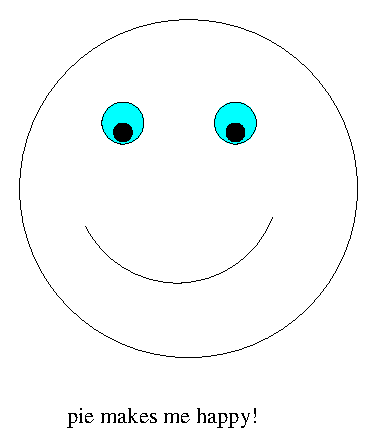
\includegraphics[width=0.4\textwidth]{fig.eps}
%%    \caption[Happy Face: figure example.]{\label{fig:happy} This is a figure of
%%      a happy face with a \texttt{psfrag} replacement.  The original figure
%%      (drawn in xfig and exported to a .eps file) has the text ``pie makes me
%%      happy!''.  The \texttt{psfrag} package replaces this with ``$\pi$ makes me
%%      happy!''.  Note: the Makefile compiles the sample using pdf\LaTeX\ which
%%      cannot use \texttt{psfrag} directly.  For some options that work with
%%      pdf\LaTeX, please see this discussion:
%%      \url{http://tex.stackexchange.com/questions/11839}.  For the caption, we
%%      have used the optional argument for the caption command so that only a
%%      short version of this caption occurs in the list of figures.}
%%  \end{center}
%%\end{figure}
%%\afterpage{\clearpage}
%%Here is an example of a figure environment.
%%Perhaps I should say that the example of a figure can be seen in
%%Figure~\ref{fig:happy}.  Figure placement can be tricky with \LaTeX\
%%because figures and tables are treated as ``floats'': text can flow
%%around them, but if there is not enough space, they will appear later.
%%To prevent figures from going too far, the
%%\verb|\afterpage{\clearpage}| command can be used.  This makes sure
%%that the figure are typeset at the end of the page (possibly appear on
%%their own on the following pages) and before any subsequent text.
%%
%%The \verb|\clearpage| forces a page break so that the figure can be
%%placed, but without the the \verb|\afterpage{}| command, the page
%%would be broken too early (at the \verb|\clearpage| statement).  The
%%\verb|\afterpage{}| command tells \LaTeX{} to issue the command after
%%the present page has been rendered.
%%
%%\section{Tables}
%%We have already included one table:~\ref{tab:Table1}.  Another table
%%is plopped right here.
%%\begin{table}[ht]
%%  \begin{center}
%%    \begin{tabular}{|l||l|l||l|l|}
%%      \hline
%%      &\multicolumn{2}{l|}{Singular}&\multicolumn{2}{l|}{Plural}\\
%%      \cline{2-5}
%%       &English&\textbf{Gaeilge}&English&\textbf{Gaeilge}\\
%%      \hline\hline
%%      1st Person&at me&\textbf{agam}&at us&\textbf{againn}\\
%%      2nd Person&at you&\textbf{agat}&at you&\textbf{agaibh}\\
%%      3rd Person&at him&\textbf{aige}&at them&\textbf{acu}\\
%%       &at her&\textbf{aici}& & \\
%%      \hline
%%    \end{tabular}
%%    \caption{
%%      \label{tab:Table2}
%%      Another table.}
%%  \end{center}
%%\end{table}
%%Well, actually, as with Figures, tables do not
%%necessarily appear right ``here'' because tables are also ``floats''.
%%\LaTeX{} puts them where it can.  Because of this, one should refer to
%%floats by their labels rather than by their location.  This example is
%%demonstrated by Table~\ref{tab:Table2}.  This one is pretty close,
%%however.  (Note: you should generally not put tables or figures in the
%%middle of a paragraph.  This example is for demonstration purposes
%%only.)
%%
%%Another useful package is \verb|\usepackage{longtable}| which provides
%%the \texttt{longtable} environment.  This is nice because it allows
%%tables to span multiple pages.  Table~\ref{tab:longtable} has been
%%formatted this way.
%%\begin{center}
%%  \begin{longtable}{|l|l|l|}
%%    \caption{\label{tab:longtable}Feasible triples for
%%      highly variable Grid}\\
%%
%%    \hline \multicolumn{1}{|c|}{\textbf{Time (s)}} &
%%    \multicolumn{1}{c|}{\textbf{Triple chosen}} &
%%    \multicolumn{1}{c|}{\textbf{Other feasible triples}} \\ \hline
%%    \endfirsthead
%%
%%    \multicolumn{3}{c}%
%%    {{\bfseries \tablename\ \thetable{} -- continued from previous page}} \\
%%    \hline \multicolumn{1}{|c|}{\textbf{Time (s)}} &
%%    \multicolumn{1}{c|}{\textbf{Triple chosen}} &
%%    \multicolumn{1}{c|}{\textbf{Other feasible triples}} \\ \hline
%%    \endhead
%%
%%    \hline \multicolumn{3}{|r|}{{Continued on next page}} \\ \hline
%%    \endfoot
%%
%%    \hline \hline
%%    \endlastfoot
%%
%%    0 & (1, 11, 13725) & (1, 12, 10980), (1, 13, 8235), (2, 2, 0), (3, 1, 0) \\
%%    274 & (1, 12, 10980) & (1, 13, 8235), (2, 2, 0), (2, 3, 0), (3, 1, 0) \\
%%    5490 & (1, 12, 13725) & (2, 2, 2745), (2, 3, 0), (3, 1, 0) \\
%%    8235 & (1, 12, 16470) & (1, 13, 13725), (2, 2, 2745), (2, 3, 0), (3, 1, 0) \\
%%    10980 & (1, 12, 16470) & (1, 13, 13725), (2, 2, 2745), (2, 3, 0), (3, 1, 0) \\
%%    13725 & (1, 12, 16470) & (1, 13, 13725), (2, 2, 2745), (2, 3, 0), (3, 1, 0) \\
%%    16470 & (1, 13, 16470) & (2, 2, 2745), (2, 3, 0), (3, 1, 0) \\
%%    19215 & (1, 12, 16470) & (1, 13, 13725), (2, 2, 2745), (2, 3, 0), (3, 1, 0) \\
%%    21960 & (1, 12, 16470) & (1, 13, 13725), (2, 2, 2745), (2, 3, 0), (3, 1, 0) \\
%%    24705 & (1, 12, 16470) & (1, 13, 13725), (2, 2, 2745), (2, 3, 0), (3, 1, 0) \\
%%    27450 & (1, 12, 16470) & (1, 13, 13725), (2, 2, 2745), (2, 3, 0), (3, 1, 0) \\
%%    30195 & (2, 2, 2745) & (2, 3, 0), (3, 1, 0) \\
%%    32940 & (1, 13, 16470) & (2, 2, 2745), (2, 3, 0), (3, 1, 0) \\
%%    35685 & (1, 13, 13725) & (2, 2, 2745), (2, 3, 0), (3, 1, 0) \\
%%    38430 & (1, 13, 10980) & (2, 2, 2745), (2, 3, 0), (3, 1, 0) \\
%%    41175 & (1, 12, 13725) & (1, 13, 10980), (2, 2, 2745), (2, 3, 0), (3, 1, 0) \\
%%    43920 & (1, 13, 10980) & (2, 2, 2745), (2, 3, 0), (3, 1, 0) \\
%%    46665 & (2, 2, 2745) & (2, 3, 0), (3, 1, 0) \\
%%    49410 & (2, 2, 2745) & (2, 3, 0), (3, 1, 0) \\
%%    52155 & (1, 12, 16470) & (1, 13, 13725), (2, 2, 2745), (2, 3, 0), (3, 1, 0) \\
%%    54900 & (1, 13, 13725) & (2, 2, 2745), (2, 3, 0), (3, 1, 0) \\
%%    57645 & (1, 13, 13725) & (2, 2, 2745), (2, 3, 0), (3, 1, 0) \\
%%    60390 & (1, 12, 13725) & (2, 2, 2745), (2, 3, 0), (3, 1, 0) \\
%%    63135 & (1, 13, 16470) & (2, 2, 2745), (2, 3, 0), (3, 1, 0) \\
%%    65880 & (1, 13, 16470) & (2, 2, 2745), (2, 3, 0), (3, 1, 0) \\
%%    68625 & (2, 2, 2745) & (2, 3, 0), (3, 1, 0) \\
%%    71370 & (1, 13, 13725) & (2, 2, 2745), (2, 3, 0), (3, 1, 0) \\
%%    74115 & (1, 12, 13725) & (2, 2, 2745), (2, 3, 0), (3, 1, 0) \\
%%    76860 & (1, 13, 13725) & (2, 2, 2745), (2, 3, 0), (3, 1, 0) \\
%%    79605 & (1, 13, 13725) & (2, 2, 2745), (2, 3, 0), (3, 1, 0) \\
%%    82350 & (1, 12, 13725) & (2, 2, 2745), (2, 3, 0), (3, 1, 0) \\
%%    85095 & (1, 12, 13725) & (1, 13, 10980), (2, 2, 2745), (2, 3, 0), (3, 1, 0) \\
%%    87840 & (1, 13, 16470) & (2, 2, 2745), (2, 3, 0), (3, 1, 0) \\
%%    90585 & (1, 13, 16470) & (2, 2, 2745), (2, 3, 0), (3, 1, 0) \\
%%    93330 & (1, 13, 13725) & (2, 2, 2745), (2, 3, 0), (3, 1, 0) \\
%%    96075 & (1, 13, 16470) & (2, 2, 2745), (2, 3, 0), (3, 1, 0) \\
%%    98820 & (1, 13, 16470) & (2, 2, 2745), (2, 3, 0), (3, 1, 0) \\
%%    101565 & (1, 13, 13725) & (2, 2, 2745), (2, 3, 0), (3, 1, 0) \\
%%    104310 & (1, 13, 16470) & (2, 2, 2745), (2, 3, 0), (3, 1, 0) \\
%%    107055 & (1, 13, 13725) & (2, 2, 2745), (2, 3, 0), (3, 1, 0) \\
%%    109800 & (1, 13, 13725) & (2, 2, 2745), (2, 3, 0), (3, 1, 0) \\
%%    112545 & (1, 12, 16470) & (1, 13, 13725), (2, 2, 2745), (2, 3, 0), (3, 1, 0) \\
%%    115290 & (1, 13, 16470) & (2, 2, 2745), (2, 3, 0), (3, 1, 0) \\
%%    118035 & (1, 13, 13725) & (2, 2, 2745), (2, 3, 0), (3, 1, 0) \\
%%    120780 & (1, 13, 16470) & (2, 2, 2745), (2, 3, 0), (3, 1, 0) \\
%%    123525 & (1, 13, 13725) & (2, 2, 2745), (2, 3, 0), (3, 1, 0) \\
%%    126270 & (1, 12, 16470) & (1, 13, 13725), (2, 2, 2745), (2, 3, 0), (3, 1, 0) \\
%%    129015 & (2, 2, 2745) & (2, 3, 0), (3, 1, 0) \\
%%    131760 & (2, 2, 2745) & (2, 3, 0), (3, 1, 0) \\
%%    134505 & (1, 13, 16470) & (2, 2, 2745), (2, 3, 0), (3, 1, 0) \\
%%    137250 & (1, 13, 13725) & (2, 2, 2745), (2, 3, 0), (3, 1, 0) \\
%%    139995 & (2, 2, 2745) & (2, 3, 0), (3, 1, 0) \\
%%    142740 & (2, 2, 2745) & (2, 3, 0), (3, 1, 0) \\
%%    145485 & (1, 12, 16470) & (1, 13, 13725), (2, 2, 2745), (2, 3, 0), (3, 1, 0) \\
%%    148230 & (2, 2, 2745) & (2, 3, 0), (3, 1, 0) \\
%%    150975 & (1, 13, 16470) & (2, 2, 2745), (2, 3, 0), (3, 1, 0) \\
%%    153720 & (1, 12, 13725) & (2, 2, 2745), (2, 3, 0), (3, 1, 0) \\
%%    156465 & (1, 13, 13725) & (2, 2, 2745), (2, 3, 0), (3, 1, 0) \\
%%    159210 & (1, 13, 13725) & (2, 2, 2745), (2, 3, 0), (3, 1, 0) \\
%%    161955 & (1, 13, 16470) & (2, 2, 2745), (2, 3, 0), (3, 1, 0) \\
%%    164700 & (1, 13, 13725) & (2, 2, 2745), (2, 3, 0), (3, 1, 0) \\
%%\end{longtable}
%%\end{center}
%%
%%\subsection*{An Unnumbered Subsection}
%%Note that if you use subsections or further divisions under an
%%unnumbered section, then you should make them unnumbered as well
%%otherwise you will end up with zeros in the section numbering.
%%
%%\chapter{Landscape Mode}
%%The landscape mode allows you to rotate a page through 90 degrees.  It
%%is generally not a good idea to make the chapter heading landscape,
%%but it can be useful for long tables etc.
%%
%%\begin{landscape}
%%  This text should appear rotated, allowing for formatting of very
%%  wide tables etc.  Note that this might only work after you convert
%%  the \texttt{dvi} file to a postscript (\texttt{ps}) or \texttt{pdf}
%%  file using \texttt{dvips} or \texttt{dvipdf} etc.  This feature is
%%  provided by the \verb|lscape| and the \verb|pdflscape| packages.
%%  The latter is preferred if it works as it also rotates the pages in
%%  the pdf file for easier viewing.
%%\end{landscape}

%% This file is setup to use a bibtex file sample.bib and uses the
%% plain style.  Other styles may be used depending on the conventions
%% of your field of study.
%%
%%% Note: the bibliography must come before the appendices.
\bibliographystyle{plain}
\bibliography{sample}

%% Use this to reset the appendix counter.  Note that the FoGS
%% requires that the word ``Appendices'' appear in the table of
%% contents either before each appendix lable or as a division
%% denoting the start of the appendices.  We take the latter option
%% here.  This is ensured by making the \texttt{appendicestoc} option
%% a default option to the UBC thesis class.

%%% If you only have one appendix, please uncomment the following line.
% \renewcommand{\appendicesname}{Appendix}
\appendix

\chapter{Terms Used}
\begin{itemize}
\item Taint: Where this is used, such as when saying that a piece of data in an application is 'tainted', it refers to data which has been tagged to be tracked by the tracking system. Whenever tainted data is detected at some monitoring point in an application, the system reports it. Taint can include information about where the data came from, as is the case for the system described here, refereed to as the 'taint source'. In this thesis is made a minor distinction between Objects which are directly tainted and those which are reachability tainted. Directly tainted Objects include a set of basic types which, once tainted, are always tainted. These include Strings, StringBuffers, StringBuilders, character arrays, and some numeric values. Reachability tainted means that a directly tainted Object is reachable through an Object's reference graph, such as by following a heirarchy of field references.
\item Tomography: This refers to the nature of the taint tracking in question. Tomography-level taint tracking is a heavy form of the analysis where tainted data is not only tagged at a source and identified at predetermined monitoring points, but is rather tracked along its complete path, indiscriminantly through many monitoring points. The basic goal of tomography is to get a complete trace of where tainted data goes in a program. 
\item Trace:
\item Flow:
\end{itemize}

\chapter{Taint Tracking Tool Logging Format}

THIS NEEDS TO BE FORMATTED, DIFFICULT TO READ\\\\
Provided here is a breakdown of the log structure that the tool uses, for reference when describing other parts of the implementation and for gauging the completeness of the tracking.

\begin{itemize}
\item location Tag \\ 
Format: <location callerClass, callerMethod, calledClass, calledMethod, requestCounter, requestURI, requestRemoteAddr, callerContextCounter, calledContextCounter /> \\
This tag appears in every log entry, and contains all information needed to determine where the event occured. The attributes of this tag are as follows: \\ 
caller/called Class/Method - these specifies the fully qualified class name and method name with argument types of the caller and callee for a particular taint flow event. For example, for a record indicating that taint was passed in the arguments of a method call, these will indicate the method from which the call was made and the called method itself.
requestCounter - this is a counter which uniquely identifies which user request a log was generated from. Everytime the application server must service a new request, a new counter value is assigned to it. \\
requestURI - the URI of the request responsible for generating a log. \\
requestRemoteAddr - the remote address (IP address of a web application user submitting a request) of the request responsible for generating a log. \\
caller/called ContextCounter - these attributes supplement the caller/called Class/Method by identifying unique instances of method calls. Every time a method call starts and the call stack changes, a new counter value is assigned to the item on top of the stack. The counters for the current caller and called methods are used when creating log records, and are useful when analysing taint flow graphs to properly determine which flows actually connect to each other.

\item Xobject Tag \\ 
Format: <Xobject type, objectID, value, taintID, taintRecord /> \\
Various 'object' tags (sourceObject, taintedObject, etc) appear in log records to describe important Objects in taint flow events. The attributes of this tag are as follows: \\
type - the Java class name for this object \\
objectID - a unique ID for the Object. We use the hashcode given by Java. \\
value - if available, a String representation of the Object. \\
taintID - an unique identifier for the taint an Object carries. If taint is propagated from one Object to another, they will have similar taintIDs (differing only by an identifier for the Object). If an Object is tainted by multiple sources, the taintID will reflect this.\\
taintRecord - See below.

\item taintRecord Attribute \\ 
Format: TARGETCOLUMN: column CATALOG: catalog TABLE: table COLUMN: column... \\
URI: uri PARAM: param \\
This attribute, found in Xobject tags for Objects carrying taint, describes where the taint originally came from. In our implementation we taint reads from databases and from user web request parameters. For database reads we log the catalog, table, and column of every column involved in the selection query, and additionally specify the target column from which the data was actually taken. For request parameters we log the URI which received the request as well as the parameter name. 

\item field Tag \\ 
Format: <field targetClass, targetField, static> \\
These tags are used in field set/get records to identify, by class and field name, the field in question. Also indicated is whether or not this is a field of a static class.

\item Propagation Log \\ 
Format: <taintlog type="PROPAGATION"><location /><sourceObject /><destObject /></taintlog> \\
Indicates that taint has spread from one Object to another. These logs mostly occur as a result of String operations, such as appending and copying, which produce new Strings from tainted ones. The sourceObject tag describes the Object which was originally tainted, and the destObject tag the one receiving taint from the sourceObject.

\item Fuzzy Propagation Log \\ 
Format: <taintlog type="FUZZY"><location /><sourceObject /><destObject /></taintlog> \\
Indicates that an Object was marked as tainted heuristically by fuzzy propagation, as described earlier. The sourceObject tag describes the Object which was originally tainted and which satisfied the levenshtein distance match with the non-tainted destObject. The destObject now carries the taint of the sourceObject.

\item Modification Log \\
Format: <taintlog type="MODIFICATION"><location /><targetObject /></taintlog> \\
Indicates that some tainted Object has been modified. This usually means that a StringBuilder/Buffer Object was changed somehow, such as by an append. The targetObject tag describes this Object.

\item Composition Log \\
Format: <taintlog type="COMPOSITION"><location tag><composedObject><composingObject />...</composedObject></taintlog> \\
Indicates that multiple tainted Objects have been combined into one Object which carries the combined taint. A composedObject tag describes the new Object, and nested inside it a series of composingObject tags describe the tainted Objects which were combined.

\item Association Log \\
Format: <taintlog type="ASSOCIATION"><location tag><associatingObjects><associatingObject />...</associatedObjects></taintlog> \\
Indicates that multiple tainted Objects have associated through certain method calls but were not combined into a single Object (such as comparing one String to another). An associatingObjects tag wraps a series of associatingObject tags describing the tainted Objects which associated.

\item Calling Log \\ 
Format: <taintlog type="CALLING"><location tag><taintedObject><subTaintedObject />...</taintedObject><callerObject /><calledObject /></taintlog> \\
Indicates that tainted Objects were passed in the arguments of a method call. For each argument which carries taint, a taintedObject tag describes the argument. If an argument is not directly tainted but from which taint is reachable, the taintedObject tag wraps a series of subTaintedObjects describing reachable directly tainted Objects. The caller/calledObject tags describe the Objects taking place in the method call.

\item Returning Log \\ 
Format: <taintlog type="RETURNING"><location tag><taintedObject><subTaintedObject />...</taintedObject><callerObject /><calledObject /></taintlog> \\
This is similar to the Calling Log, but indicates that a tainted Object has been returned from a method call.

\item Returning Args Log \\ 
Format: <taintlog type="RETURNINGARGS"><location tag><taintedObject><subTaintedObject />...</taintedObject><callerObject /><calledObject /></taintlog> \\
This is similar to the Calling Log, but comes when the method is returning and indicates that arguments have taken on additional taint as a result of the method execution.

\item Returning Input Log \\ 
Format: <taintlog type="RETURNINGINPUT"><location tag><taintedObject><subTaintedObject />...</taintedObject><callerObject /><calledObject /></taintlog> \\
This is similar to the Returning Log, but is used for special cases to indicate that a return value is an original source of tainted data, such as a read operation from a database Object.

\item Output Log \\ 
Format: <taintlog type="OUTPUT"><location tag><taintedObject><subTaintedObject />...</taintedObject><callerObject /><calledObject /></taintlog> \\
This is similar to the Calling Log, but is used for special cases to indicate that the arguments will be output to some important location, such as back to the user as web page text, or into a database.

\item Non-Taint Output Log \\ 
Format: <taintlog type="NONTAINTOUTPUT"><location tag><outputObject /><callerObject /><calledObject /></taintlog> \\
This is similar to the Output Log, and is used in the same cases as it where the output data is not tainted. This allows one to see how tainted and non-tainted data mix in the output of the application.

\item Field Set Log \\
Format: <taintlog type="FIELDSET"><location tag><field /><taintedObject><subTaintedObject />...</taintedObject><callerObject /><calledObject /></taintlog> \\
This is similar to the Calling Log, but indicates that a tainted Object has been assigned to an Object or static class field.

\item Field Get Log \\
Format: <taintlog type="FIELDGET"><location tag><field /><taintedObject><subTaintedObject />...</taintedObject><callerObject /><calledObject /></taintlog> \\
This is similar to the Returning Log, but indicates that a tainted Object has been read from an Object or static class field.

% This log type may not be needed if we replace it with FIELDSET records.
%\item Static Field Store Log \\ t

\end{itemize}
%Here you can have your appendices.  Note that if you only have a
%single appendix, you should issue
%\verb|\renewcommand{\appendicesname}{Appendix}| before calling
%\verb|\appendix| to display the singular ``Appendix'' rather than the
%default plural ``Appendices''.

\chapter{Second Appendix}
Here is the second appendix.

%% This changes the headings and chapter titles (no numbers for
%% example).
\backmatter

%% Indices come here if you have them.

%%\chapter*{Additional Information}
%%This chapter shows you how to include additional information in your
%%thesis, the removal of which will not affect the submission.  Such
%%material should be removed before the thesis is actually submitted.
%%
%%First, the chapter is unnumbered and not included in the Table of
%%Contents.  Second, it is the last section of the thesis, so its
%%removal will not alter any of the page numbering etc. for the previous
%%sections.  Do not include any floats, however, as these will appear in
%%the initial lists.
%%
%%The \texttt{ubcthesis} \LaTeX{} class has been designed to aid you in
%%producing a thesis that conforms to the requirements of The
%%University of British Columbia Faculty of Graduate Studies (FoGS).
%%
%%Proper use of this class and sample is highly recommended---and should
%%produce a well formatted document that meets the FoGS requirement.
%%Notwithstanding, complex theses may require additional formatting that
%%may conflict with some of the requirements.  We therefore \emph{highly
%%  recommend} that you consult one of the FoGS staff for assistance and
%%an assessment of potential problems \emph{before} starting final
%%draft.
%%
%%While we have attemped to address most of the thesis formatting
%%requirements in these files, they do not constitute an official set of
%%thesis requirements.  The official requirements are available at the
%%following section of the FoGS web site:
%%\begin{center}
%%  \begin{tabular}{|l|}
%%    \hline
%%    \url{http://www.grad.ubc.ca/current-students/dissertation-thesis-preparation}\\
%%    \hline
%%  \end{tabular}
%%\end{center}
%%We recommend that you review these instructions carefully.

\end{document}
\endinput
%%
%% End of file `ubcsample.tex'.
